\documentclass[12pt,a4paper,twoside,openright]{report}

\usepackage{algpseudocode,algorithm}			% alghoritms and pseudocode
\usepackage{listings}						% code snippets
\usepackage{amsmath,amsfonts,amsthm,amssymb}	% math stuff
\usepackage{fancyhdr}						% control page header and footer
\usepackage{hyperref}
\usepackage{array}							% tabular and array utils
\usepackage{lscape}							% for landscape placement
\usepackage{graphicx}						% for images
\usepackage[english]{babel}					% language support
\usepackage[nottoc]{tocbibind}				% bibliography to toc
\usepackage{color}
\usepackage{float} % for floating objects

\definecolor{light-gray}{gray}{0.95}
\definecolor{yellow}{RGB}{255, 251, 140}

% defining single line code blocks with monospace font and light-gray backgounf
\newcommand{\code}[1]{\colorbox{light-gray}{\texttt{#1}}}
% note command
\newcommand{\todo}[1]{\colorbox{yellow}{\textbf{\#TODO} #1}}

\pagestyle{fancy}

\sloppy
\raggedbottom

\linespread{1.5}
% \renewcommand{\baselinestretch}{1.3}

\makeatletter
\def\cleardoublepage{\clearpage\if@twoside \ifodd\c@page\else
\hbox{}
\vspace*{\fill}
\begin{center}
	% this page intentionally contains only this sentence.
\end{center}
\vspace{\fill}
\thispagestyle{empty}
\newpage
\if@twocolumn\hbox{}\newpage\fi\fi\fi}
\makeatother

%------------------------------------------------------
% hyphenation settings
%------------------------------------------------------
\lefthyphenmin=4
\righthyphenmin=4
\tolerance=1000
\hyphenpenalty=100
\emergencystretch=1cm
\widowpenalty=5000
\clubpenalty=2500

%--------------------------------------------------------
% pages size setup
%--------------------------------------------------------
\renewcommand{\headrulewidth}{0.5pt}
\hoffset=-15mm
%\topmargin=0mm
\headheight=15pt
\textwidth=140mm
\headsep=5mm
\voffset=-5mm
%\hsize=13cm
%\textwidth=164mm
\textheight=230mm
\evensidemargin=25mm
\oddsidemargin=25mm
%\marginparwidth=0mm

%--------------------------------------------------------------
% page headers setup
%--------------------------------------------------------------
\pagestyle{fancy}
\renewcommand{\chaptermark}[1]{\markboth{#1}{}}
\renewcommand{\sectionmark}[1]{\markright{\thesection\ #1}}
\fancyhf{}
\fancyfoot[LE,RO]{\bfseries\thepage}
\fancyhead[RO]{\bfseries\rightmark}
\fancyhead[LE]{\bfseries\leftmark}
\fancypagestyle{plain}{
\fancyhead{}
\fancyfoot{}
\renewcommand{\headrulewidth}{0pt}
}

%--------------------------------------------------------------------------------
% custom commands %--------------------------------------------------------------------------------
\newcommand{\newparagraph}{\noindent\\}
\newcommand{\xmark}{\ding{55}}
\newcommand{\cmark}{\ding{51}}

%--------------------------------------------------------------------------------
% document start
%--------------------------------------------------------------------------------
\begin{document}

\pagenumbering{roman}
\setcounter{page}{1}
\pagestyle{empty}

%--------------------------------------------------------------------------------
% listings configiuration
%--------------------------------------------------------------------------------
\lstset{
	frame=tb,
	captionpos=b,
	basicstyle=\footnotesize,
	numbers=left,
	aboveskip=1em
}

%--------------------------------------------------------------------------------
% include title page
%--------------------------------------------------------------------------------
\begin{titlepage}
 \begin{center}
 
\includegraphics[width=3cm]{images/logo_polimi.png}
 {\begin{center}
 \begin{LARGE}
 \textbf{\uppercase{politecnico di milano}}
 \end{LARGE}
 \begin{large}
 \textsc{
 dipartimento di elettronica, informazione e bioingegneria
 }
 \end{large}
 \end{center}
 }
 \vspace*{0.3cm}
 {\Large 
 \emph{Corso di Laurea Magistrale in Ingegneria Informatica\\[1.3cm]}
 }
 % \vfill
 \begin{Huge}
 \textbf{Towards Virtual Machine\\[0.4cm]
 Consolidation in OpenStack
 }
 \end{Huge}
 \vfill
 \begin{minipage}{.99\linewidth}
 \begin{tabular}{l r}
 \begin{minipage}{.4\linewidth}
 \begin{flushleft}
 {\large
 RELATORE\\[.3cm]
 Prof. Sam Jesus Alejandro GUINEA MONTALVO
 }
 \end{flushleft}
 \end{minipage}
 &
 \begin{minipage}{.6\linewidth}
 \begin{flushright}
 {\large
 TESI DI LAUREA DI\\[.3cm]
 Lorenzo AFFETTI\\
 Matr. 799284\\[.3cm]
 Giacomo BRESCIANI\\
 Matr. 804979
 }
 \end{flushright}
 \end{minipage}
 \end{tabular}
 \end{minipage}
 \vfill
 {\large{{Anno Accademico 2013/2014}}}
 \end{center}
\end{titlepage}
\cleardoublepage

%--------------------------------------------------------------------------------
% dedica
%--------------------------------------------------------------------------------
\thispagestyle{empty}

\begin{flushright}
\Large\textit{dedica\dots}
\end{flushright}

%\null\vfil

\cleardoublepage

%--------------------------------------------------------------------------------
% ringraziamenti
%--------------------------------------------------------------------------------
\thispagestyle{empty}

\chapter*{Ringraziamenti}

\begin{flushleft}
Milano, 1 Aprile 2005
\end{flushleft}

\begin{flushright}
\emph{Affear}
\end{flushright}

\cleardoublepage
\thispagestyle{empty}

\pagestyle{fancy}
\renewcommand{\contentsname}{Table of Contents}%

%--------------------------------------------------------------------------------
% talbe of contents
%--------------------------------------------------------------------------------
\tableofcontents
\cleardoublepage
\listoffigures
\listoftables
%\listofalgorithms
%\lstlistoflistings

\pagenumbering{arabic}

\setcounter{page}{1}

%--------------------------------------------------------------------------------
% Introduction
%--------------------------------------------------------------------------------
\chapter{Introduction}
\label{chap:intro}
%!TEX root = ../thesis.tex
%%--------------------------------------------------------------------------
%% INTRODUCTION
%%--------------------------------------------------------------------------

The problem of resources allocation, in the past years, has increasingly attracted the attention of the community for its important implications in the field of energy saving. The rapid growth of cloud services has in fact heavily raised the number of data centers all over the world, consequentially increasing their power consumption. Nowadays, data centers energy consumption has indeed become a really urgent and important problem as the power they need has reached the \% of the world's total in \todo{\% year and reference}.\\
For that reason, an intelligent and efficient strategy for resources allocation is critical to try to make the most of available hardware. Within a IaaS, one way to achieve this goal is try to have the minimum number of running servers while maintaining all the virtual machines which were requested from the users running and available. This is commonly done through an intelligent \textit{VMs Placement} on available servers when a VM is requested. Exploiting this solution it is possible to ensure that the data center is ``filled'' in a consistent way, avoiding under-allocated resources.\\
The problem with the previous solution is that it doesn't cover those cases in which VMs are deallocated from the hosting hardware. In these cases, in fact, the system could reach a state where all the data center servers are no more used efficiently, leaving some of them, for example, under-utilized, and so consuming more power than needed. To address this problem it is possible to \textit{consolidate} the arrangement of VMs within the data center, migrating them from under-utilized servers to servers which can host them; thanks to this migrations it will be possible to ``empty'' these under-utilized machines and take them in an energy-saving power state, such as deep-sleep. This process is called \textit{VMs Consolidation} and it is  very interesting way to increase power saving. In fact, as deepen in the State of the Art chapter (see \ref{chap:sota}), during the past years VMs Consolidation has gained more and more attention from the community, and a lot of algorithms and technique were proposed to address it in the best way.\\
However, despite it is one of the more interesting approach to power saving, VMs Consolidation lacks of implementations, especially in non-proprietary IaaS , and the majority of the solutions are mostly theoretical without practical tests in real environments. For example OpenStack (see chapter \ref{chap:openstack_devstack}), the most important and used IaaS open-source solution doesn't provide an official implementation or a way to exploit VMs consolidation.

 
At the beginning of the development of the thesis we were mainly focused on the implementation of a module for OpenStack that would allow us to implement different consolidation algorithms and to test them to see their impact on a real cloud system, in terms of resource allocation. At the beginning we faced the problem of running, testing and benchmarking our code in an OpenStack environment. Indeed to deal with aspects like Scheduling, Virtual Machines Placement, and Server Consolidation we needed an highly configurable system that would allow us to run simulations and benchmarks to evaluate the soundness of our solutions.\\ 
A common barrier to experimenting with cloud infrastructure is in fact the lack of access to a fully functional cloud installation. Although OpenStack can be used to create testbeds, it is not uncommon in literature to find works that are plagued by unrealistic setups that use only a handful of servers. Moreover, setting up a testbed is necessary but not sufficient. One must also be able to create repeatable experiments that can be used to compare one’s results to baseline or related approaches from the state of the art.
So we designed and develop a system to address this problem: we wanted it to be fully customizable to match different requirements and let the user customize a lot of aspects, such as the structure of the environments, the number of Compute Nodes (the nodes that host Virtual Machines), their fake characteristics (see section \ref{sec:openstack_fake_drivers} on \code{FakeDrivers}) or the OpenStack services to run. Secondly we needed a way to automatically simulate, in a repeatable way, the workload generated from user applications that normally run on an OpenStack installation. At last we realized that it would be very useful to show the real time data of the simulations to analyze the behavior of the system in different configurations.
Therefore we decided to develop aDock, a suite of tools for creating performance, sandboxed, and configurable cloud infrastructure experimentation environments that developer, sysadmins and researchers can exploit to access a fully functional cloud installation of OpenStack.


%--------------------------------------------------------------------------------
% OpenStack and DevStack
%--------------------------------------------------------------------------------
\chapter{OpenStack and DevStack}
\label{chap:openstack_devstack}
%!TEX root = ../thesis.tex
%%--------------------------------------------------------------------------
%% OPENSTACK AND DEVSTACK
%%--------------------------------------------------------------------------


In this chapter we are going to present OpenStack and DevStack; we shall provide a brief overview and focus on the components and aspects that most concern the topics of our thesis.

\section{OpenStack}
\label{sec:openstack}
OpenStack is an open-source cloud computing software platform that provides a complete IaaS solution for public and private clouds. Founded by Nasa\footnote{\url{www.nasa.gov} (2015)} and Rackspace Cloud\footnote{\url{www.rackspace.com} (2015)} in 2010 OpenStack is now one of the biggest open-source projects with more than twenty thousand people working on it and more than twenty million code lines. It is a cloud operating system that controls large pools of compute, storage, and networking resources throughout a datacenter (with the possibility of controlling them trough a dashboard) and enabling enterprises and service providers to offer on-demand computing resources.\\
One of its main strengths is its modularity, which provides the flexibility needed to design different configurations for different cloud environments; its core components are:
\begin{description}
	\item[Compute] The service called \texttt{Nova} is the primary computing engine and it is used to deploy and manage large numbers of Virtual Machines.
	\item[Storage] The storage platform, divided in Object Storage (\texttt{Swift}) and Block Storage (\texttt{Cinder}).
	\item[Network] The service called \texttt{Neutron} offers Networking as a Service
	\item[Dashboard] \texttt{Horizon} that is a dashboard provides users with a graphical user interface to access, provision, and automate cloud-based resources.
	\item[Shared Services] Other services, that makes it easier to manage the IaaS, such as the Identity Service (\texttt{Keystone}), the Image Service (\texttt{Glance}), Telemetry (\texttt{Ceilometer}), Orchestration (\texttt{Heat}) and others.
\end{description}

\begin{figure}[!ht]
\centering{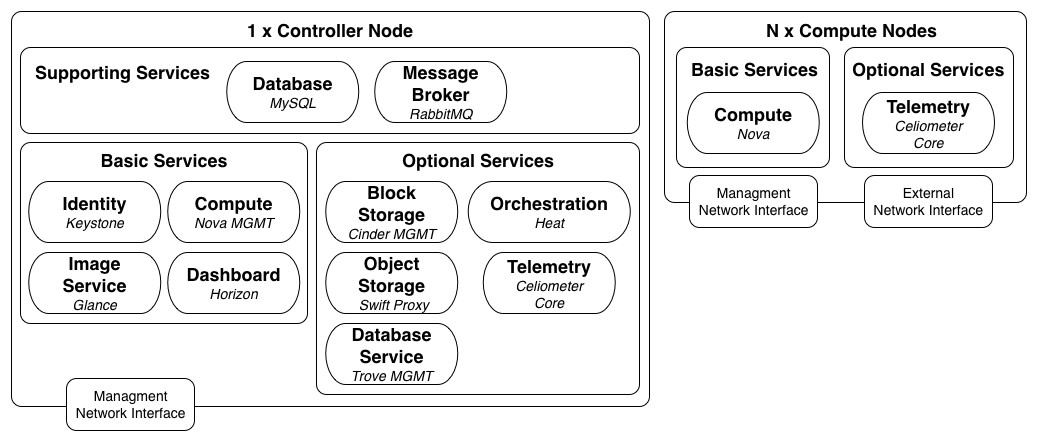
\includegraphics[width=\textwidth]{images/openstack_arch.png}}
\label{fig:openstack_1plusN}
\caption{A ``1 + N'' OpenStack configuration}
\end{figure}

We have decided to focus on the creation of ``1 + N'' installations of OpenStack; these are composed of one \textit{Controller} node and N \textit{Compute} nodes with legacy networking. Legacy networking refers to a basic solution in which we do not deploy \texttt{Neutron} but we exploit \code{nova-network}, a \texttt{Nova} service described in paragraph \ref{par:openstack_nova_net}. The figure~\ref{fig:openstack_1plusN} on page~\pageref{fig:openstack_1plusN} provides a high level view of all the OpenStack services, both basic and optional, that have to be installed both on the Controller and the Compute nodes to setup a ``1 + N'' configuration.\\ 
The Controller node is responsible for globally managing the cloud operations. It runs the user \texttt{Identity} service, the Virtual Machine \texttt{Image} service, the management portion of the \texttt{Compute} service, and a \textit{Dashboard} through which the users can request the creation of new Virtual Machines. Optionally, the node can run the management portions of the \texttt{Block}, \texttt{Object}, and \texttt{Database Storage} services, and the \texttt{Telemetry} and \texttt{Orchestration} services. The Controller node also runs a series of supporting services (i.e., the \texttt{Database} and \texttt{Message Broker} services). Each of the N basic Compute nodes, on the other hand, runs the \texttt{Compute} service and optionally the \texttt{Telemetry} service.

\subsection{Nova}
\label{sec:openstack_nova}
OpenStack Compute module, \texttt{Nova}, is the core of OpenStack; it takes care of deploying and managing Virtual Machines, by placing them on physical machines, letting them communicate, storing their informations on an SQL database, and offering a set of HTTP managed APIs and a command-line client.
In the next paragraphs we will briefly describe the three \texttt{Nova} sub-modules that are relevant for our work.

\subparagraph{Nova-compute}
\label{par:openstack_nova_compute}
The \texttt{nova-compute} is the sub-module that takes care of booting, resizing, live-migrating and destroying the Virtual Machines that are running on the physical servers, and of letting them communicate with the hypervisor.\\
Hereunder are reported four examples of the main commands (also accessible through the Nova APIs) used to boot, resize, destroy and live-migrate Virtual Machines:
\begin{itemize}
	\item \code{\$ nova boot --flavor <flavor> --image <image>}
	\item \code{\$ nova resize --flavor <vm> <flavor>}
	\item \code{\$ nova delete <vm>}
	\item \code{\$ nova live-migration <vm> <host>}
\end{itemize}

\subparagraph{Nova-network}
\label{par:openstack_nova_net}
\texttt{Nova-network} is the basic network management module of OpenStack. It i included directly in \texttt{Nova}. Unlike \texttt{Neutron}, which can virtualize and manage both layer 2 (logical) and layer 3 (network) of the OSI network, \texttt{nova-network} only provides layer 3 virtualization and has some limitations on the network topology.\\
However \texttt{nova-network} is still supported by OpenStack and in powerful enough to support a ``1 + N'' configuration. It also streamlines the installation process as it avoids having to install another service (\texttt{Neutron}) and its dependencies.

\subparagraph{Nova-scheduler}
\label{par:openstack_nova_sched}
\texttt{Nova} uses the \texttt{nova-scheduler} service to determine how to dispatch compute requests. It is used, for example, to determine on which host a Virtual Machine should launch. The system administrator can modify and configure the \code{/etc/nova/nova.conf} configuration file to adjust the criteria under which the \texttt{nova-scheduler} will place the Virtual Machines. The process of placing Virtual Machines on the most suitable host is divided in a \textit{filtering} step, in which a list of candidate hosts is generated, and a \textit{weighing} step in which the list is ordered according to the selected criteria and the best host is chosen.

\subsection{Fake Drivers}
\label{sec:openstack_fake_drivers}
To deal with situations in which the compute nodes are not physical machines that will host real Virtual Machines, but they have be ``fake'' in the sense that they don't host a real hypervisor, OpenStack offers a module called \code{nova.virt.fake} that allows developers, that don't have real hardware, to test \code{Nova} code on compute nodes without a real hypervisor such as \textit{libvirt}. When exploiting this solution Virtual Machines, are mere python objects; in such a way the Virtual Machines are not really spawned but simply stored in the database. However \code{FakeDriver} mimics the correct behavior of a real hypervisor, allowing one to test the rest of the \code{Nova} running flow.\\
This module is not configurable and by default a \code{FakeDriver} offers 1000 VCUs, 800000 MB of RAM, and 600000 GB of Hard Disk. 

\section{DevStack}
\label{sec:devstack}
 
DevStack\footnote{More info at \url{docs.openstack.org/developer/devstack}} is a set of scripts and utilities to quickly deploy an OpenStack cloud environment and it is freely available on GitHub\footnote{\url{github.com/openstack-dev/devstack}}.\\
DevStack allows developers and system administrators to automate the process of installing OpenStack on a server reducing it to a simple command for every installation.\\
The services that are configured by default are Identity (\texttt{Keystone}), Object Storage (\texttt{Swift}), Image Storage (\texttt{Glance}), Block Storage (\texttt{Cinder}), Compute (\texttt{Nova}), Network (\texttt{Nova}), Dashboard (\texttt{Horizon}) and Orchestration (\texttt{Heat}).
The main script is \code{stack.sh}; all the required configurations, such as the Git repositories to use, the services to enable or the OS images to use, can be achieved overriding default environment variables (found in \code{stackrc}) through file \code{local.conf}. This is achieved with a \code{localrc} section, as shown below:
\begin{lstlisting}[numbers=none,label={lst:devstack_local_conf}]
[[local|localrc]]
ADMIN_PASSWORD=secrete
DATABASE_PASSWORD=$ADMIN_PASSWORD
RABBIT_PASSWORD=$ADMIN_PASSWORD
SERVICE_PASSWORD=$ADMIN_PASSWORD
SERVICE_TOKEN=a682f596-76f3-11e3-b3b2-e716f9080d50
# ...
ENABLED_SERVICES=n-cpu,n-api,n-net
# ...
\end{lstlisting}
The environment variable \code{ENABLED\_SERVICES} is used to define the service to run: in listing \ref{lst:devstack_local_conf} the \texttt{Nova} services to install, in a simple compute node installation, are \texttt{nova-compute}, \texttt{nova-api}, \texttt{nova-network}.
By running the script \code{tools/install\_prereqs.sh} it is furthermore possible to install all the dependencies required by the configured services.\\Other useful scripts provided by DevStack are \code{unstack.sh}, that allows to stop everything that was started by \code{stack.sh}, and \code{clean.sh} that tries to remove all the traces left by the OpenStack installation performed by DevStack.


%--------------------------------------------------------------------------------
% State of the art
%--------------------------------------------------------------------------------
\chapter{State of the art}
\label{chap:sota}
%!TEX root = ../thesis.tex
%%--------------------------------------------------------------------------
%% STATE OF THE ARTS
%%--------------------------------------------------------------------------



% --------------------------------------------------------------------------- %
% ---------------------------------- INTRO ---------------------------------- %
% --------------------------------------------------------------------------- %


\section{Introduction}
\label{sec:sota_intro}
At the beginning of the development of the thesis we were mainly focused on the implementation of a module for OpenStack that would allow us to implement different consolidation algorithms and to test them to see their impact on a real cloud system, in terms of resource allocation. At the beginning we faced the problem of running, testing and benchmarking our code in an OpenStack environment. Indeed to deal with aspects like Scheduling, Virtual Machines Placement, and Server Consolidation we needed an highly configurable system that would allow us to run simulations and benchmarks to evaluate the soundness of our solutions.\\ 
A common barrier to experimenting with cloud infrastructure is in fact the lack of access to a fully functional cloud installation. Although OpenStack can be used to create testbeds, it is not uncommon in literature to find works that are plagued by unrealistic setups that use only a handful of servers. Moreover, setting up a testbed is necessary but not sufficient. One must also be able to create repeatable experiments that can be used to compare one’s results to baseline or related approaches from the state of the art.
So we designed and develop a system to address this problem: we wanted it to be fully customizable to match different requirements and let the user customize a lot of aspects, such as the structure of the environments, the number of Compute Nodes (the nodes that host Virtual Machines), their fake characteristics (see section \ref{sec:openstack_fake_drivers} on \code{FakeDrivers}) or the OpenStack services to run. Secondly we needed a way to automatically simulate, in a repeatable way, the workload generated from user applications that normally run on an OpenStack installation. At last we realized that it would be very useful to show the real time data of the simulations to analyze the behavior of the system in different configurations.
Therefore we decided to develop aDock®, a suite of tools for creating performance, sandboxed, and configurable cloud infrastructure experimentation environments that developer, sysadmins and researchers can exploit to access a fully functional cloud installation of OpenStack.
For that reason this chapter is divided into two sections that present the state of the arts of Virtual Machines Consolidation and of Cloud test environments.


% ------------------------------------------------------------------------- %
% --------------------------- VMs consolidation --------------------------- %
% ------------------------------------------------------------------------- %

\section{Virtual Machine consolidation}
\label{sec:sota_vm_cons}

At its most basic essence, cloud computing can be seen as a means to provide developers with computation, storage, and networking resources on-demand, using virtualization techniques and the service abstraction \cite{Armbrust:2010ee}. The service abstraction makes the cloud suitable for use in a wide variety of scenarios, allowing software developers to create unique applications with very small upfront investments, both in terms of capital outlays and in terms of required technical expertise. Thanks to Cloud Computing, Internet software services have rightfully taken their place as important enablers in areas of great social importance, such as ambient assisted living \cite{Zhang:2011dq}, education \cite{Sultan:2010fd}, social networking \cite{Chard:2010eh}, and mobile applications \cite{Fernando:2013ip}.\\
Managing a Cloud Infrastructure, however, presents many unique challenges. For example, there has been a lot of focus in the last few years on Virtual Machines Placement and Server Consolidation, given the role they play in optimizing resource utilization and energy consumption \cite{Feller:2012kf}, \cite{Goudarzi:2012gw}. Virtual Machine (VM) Placement \cite{Meng:2010im}, \cite{Xu:2010df} defines how a cloud installation decides on which physical server to create a new virtual machine, when one is requested. Server Consolidation techniques \cite{Wuhib:2012vq}, \cite{Corradi:2014fe}, on the other hand, allow a cloud provider to perform periodical run-time optimizations, for example through the live migration of VMs. The goal is always to desist from having too many under-utilized hardware resources given a specific workload, and to achieve this without compromising the quality of service that is offered to the cloud’s customers.\\
Dynamic consolidation of Virtual machines is enabled by \textit{live migration}, that is the capability to move a running Virtual Machine from one physical hosts to another with no downtime and no disruptions for the user. Thanks to dynamic Virtual Machine consolidation it is possible to minimize the number of active hosts, and to remove Virtual Machines from hosts when they become overloaded therefore avoiding performance degradation.

With regard to Virtual Machine Consolidation a lot of solutions, algorithms and techniques have been proposed in literature \cite{He:2012jr}, \cite{Wuhib:2012vq}, \cite{Corradi:2014fe}; we decided to focus on four interesting papers described in sections \ref{sec:sota_ga}, \ref{sec:sota_holistic}, \ref{sec:sota_game_theroy} and \ref{sec:sota_mutli_agent}. The section \ref{sec:sota_neat} is dedicated to the only attempt within the state of the art to apply Virtual Machine consolidation in the OpenStack world.

\subsection{Genetic Algorithm}
\label{sec:sota_ga}
In the paper \textit{Toward Virtual Machine Packing Optimization Based on Genetic Algorithm}\cite{Nakada:2009in} the authors explain how they modeled the problem of Virtual Machines consolidation as a bin packing problem and how they structured a Genetic Algorithm to deal with it. A Genetic Algorithm is a heuristic algorithm, i.e., a type of technique that is often used to address NP-hard problems such as the bin packing problem. A GA is a kind of machine learning that takes inspiration from the concept of evolution observed in biological environments, from which it borrows a lot of terms such as Chromosome, Mutation or Population.\\
The paper in question defines the concepts of a Genetic Algorithm for the Virtual Machine packing problem as follows:
\begin{description}
  \item[Chromosome] It represents a physical node, and in particular the list of hosted virtual machines.
  \item[Crossover] They use a One-Point Crossover that randomly cuts two chromosomes and mix them. They also implement a repair function to fix the inconsistent children thus obtained.
  \item[Mutation] They randomly exchange two positions between them.
  \item[Initial Population Generation] They generate the initial population using a Minimal Generation Gap method.
  \item[Objective Function] The unspecified objective function is said to be designed with parameters and weights in mind, such as SLA (Service level agreement) violations, number of active nodes, and number of migrations applied.
\end{description}

The experimentation environment and the simulation tests are not described in a detailed way and there are no data results to prove the soundness of the approach. Still, the idea of implementing a Genetic Algorithm to solve the consolidation problem is interesting, and possibly very efficient and useful; for these reasons we decided to take inspiration from it and implement a Genetic Algorithm, to be applied in an OpenStack test environment deployed with aDock, as described in section \ref{sub:algs_ga}.

\subsection{Holistic Approach}
\label{sec:sota_holistic}
The paper \textit{Energy Management in IaaS Clouds: A Holistic Approach} published during the IEEE Fifth International Conference on Cloud Computing in 2012 presents energy management algorithms and a holistic energy-aware Virtual Machine management framework for private clouds called Snooze.\\
The system architecture described by the authors (see figure \ref{fig:snooze_arch} on page \pageref{fig:snooze_arch}) is divided in three layers:
\begin{description}
  \item[Physical layer] It contains clusters of nodes; each is controlled by a Local Controller (LCs).
    \begin{itemize}
      \item \textit{Local Controller} - They enforce Virtual Machines and host management commands coming from the GM (Group Manager, see below). Moreover, they monitor VMs, detect overload/underload anomalous situations and report them to the assigned GM.
    \end{itemize}
  \item[Hierarchical layer] It allows to scale the system and is composed of fault-tolerant components: Group Managers (GMs) and a Group Leader (GL).
      \begin{itemize}
      \item \textit{Group Leader} - One GL oversees the GMs, keeps aggregated GM resource summary information, assigns LCs to GMs, and dispatches VM submission requests to the GM.
      \item \textit{Group Managers} - Each of them manages a subset of physical hosts; they retrieve resource information and send commands, received by the GL, to the LCs.
      \end{itemize}
  \item[Client layer] It provides the user interface and it is implemented by a predefined number of replicated Entry Points (EPs).
\end{description}

The system addresses the scheduling problem both at the GL level, where VM to GM dispatching is done based on the GM resource summary information in a round-robin way, and at the GM level where the real scheduling decisions are made. In addition to the \textit{placement policies}, which are applied when a new VM is requested, the work also supports \textit{relocation policies}, which are called when overload or underload events arrive from LCs, and \textit{consolidation policies}, which are called periodically according to one interval that is specified by the system administrator.\\
The paper proposes an algorithm for both overload and underload relocation policy. They both take as input the overloaded/underloaded LC along with its associated VMs and a list of LCs managed by the GM and output a Migration Plan (MP) which specifies the new VM locations.\\
The algorithm proposed for the consolidation follows an all-or-nothing approach and attempts to move VMs from the least loaded LC to a non-empty LC with enough spare capacity.  LCs are first sorted in decreasing order based on their estimated utilization. Afterwards, VMs from the least loaded LC are sorted in decreasing order, placed on the LCs starting from the most loaded one and added to the migration plan. If all VMs could be placed the algorithm increments the number of released nodes and continues with the next LC. Otherwise, all placed VMs are removed from the LC and MP and the procedure is repeated with the next loaded LC. The algorithm terminates when it has reached the most loaded LC and outputs the MP, number of used nodes, and number of released nodes\cite[p.~208]{Feller:2012kf}.\\
In section \ref{sub:algs_holistic} we describe how we implemented this algorithm in our system and the result obtained with our configuration.


\begin{figure}[!ht]
\centering{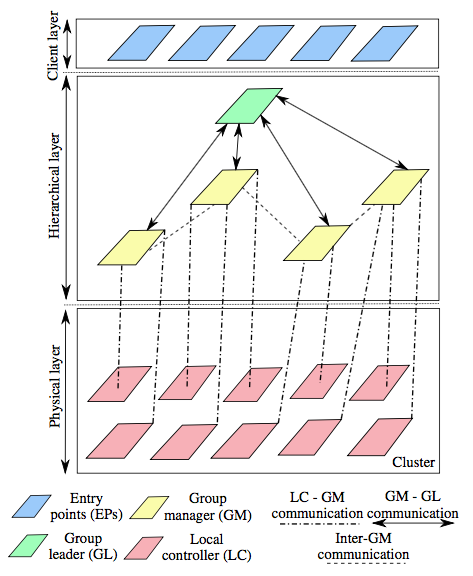
\includegraphics[width=\textwidth]{images/snooze_arch.png}}
\label{fig:snooze_arch}
\caption{The Snooze architecture \cite{Feller:2012kf}}
\end{figure}

\subsection{Game Theory Approach}
\label{sec:sota_game_theroy}
The paper \textit{A Game Theory Approach to Fair and Efficient Resource Allocation in Cloud Computing} proposes a game theoretic resources allocation algorithm that considers the fairness among users and the resources utilization for both \cite{Xu:2014do}.\\
The four main components of the proposed cloud resource management system are:
\begin{description}
  \item[CEM - Cloud Environment Monitor] This component retrieves information like host names and IP addresses about physical servers, and monitors their statuses (starting, running, shutdown) and the consumption of CPU, memory, and disk storage.
  \item[RC - Register Center] Every physical server in cloud data center should register its information to RC for connection and management.
  \item[IM - Infrastructure Manager] It is responsible for deploying and managing the virtualized infrastructures, such as creating and releasing virtual machines.
  \item[CC - Control Center] It is the control center to provide the most appropriate decision about resource allocating.
\end{description}

CEM monitors the statuses and resource consumptions for physical servers registered in RC. Once a new physical server joins the cloud, information like its MAC address and its IP address will be registered to RC. When a user sends a service request to the cloud, the resource requirements this request will be received by CC. CC makes an intelligent resource allocation decision based on the information collected by CEM. The allocation decision is executed by IM to manage the physical servers and place the virtual machines.\cite[p.~3]{Xu:2014do}

They experimented a FUGA (Fairness-Utilization tradeoff Game Algorithm) on a server cluster composed of 8 nodes and compared it to the Hadoop\footnote{A framework that allows for the distributed processing of large data sets across clusters of computers using simple programming models. \url{http://hadoop.apache.org}} \textit{fair scheduler}\footnote{``Fair scheduling is a method of assigning resources to jobs such that all jobs get, on average, an equal share of resources over time.'', \url{hadoop.apache.org/docs/r1.2.1/fair_scheduler.html}}. They showed that it is possible to achieve an optimal tradeoff between fairness and efficiency compared with the evaluation of the Hadoop scheduler.

\subsection{Multi-agent Virtual Machine Management}
\label{sec:sota_mutli_agent}
The solution presented in the paper \textit{Multi-agent Virtual Machine Management Using the Lightweight Coordination Calculus} specifies the migration behavior of Virtual Machines within, and between cloud environments. It uses a Lightweight Coordination Calculus to provide an executable, declarative specification of an agent interaction model\cite{Anderson:2013bh}.

The proposed system is distributed between nodes; it doesn't have a central controller that could represent a single point of failure or a bottleneck. Agents located on the physical machines negotiate VM transfer between themselves, without referencing any centralized authority\cite[p.~124]{Anderson:2013bh}.

The framework designed by the authors provides different types of interaction models by which it is possible to implement a wide range of algorithms and policies to support different situations.

\subsection{Neat}
\label{sec:sota_neat}
OpenStack, at the state of the art, provides a comprehensive and efficient Virtual Machines Placement system. As described in section \ref{par:openstack_nova_sched}, it is part of the \code{nova-scheduler} module. However, with regard to Virtual Machines Consolidation, OpenStack does not include any official solution or plans to include it.\\
The only project that tried to bring Virtual Machine consolidation concepts to OpenStack is Neat\footnote{\url{github.com/beloglazov/openstack-neat}}. It is defined as a framework for dynamic and energy-efficient consolidation of virtual machines in OpenStack clouds \cite{beloglazov2014openstack}.\\
OpenStack Neat approaches the consolidation problem by splitting it in four sub-problems~\cite[p.~3]{beloglazov2014openstack}:
\begin{itemize}
  \item  Deciding whether a host is \textit{underloaded}. In this case all Virtual Machines should be migrated from it, and the host should be switched to a low-power mode. 
  \item Deciding whether a host is \textit{overloaded}. In this case some Virtual Machines should be migrated from it to an other active host or a host should be reactivated to avoid violating the QoS requirements.
  \item Selecting the Virtual Machines to migrate from an overloaded host.
  \item Placing the selected Virtual Machines on an other active host, or on a reactivated one.
\end{itemize}

\begin{figure}[!ht]
\centering{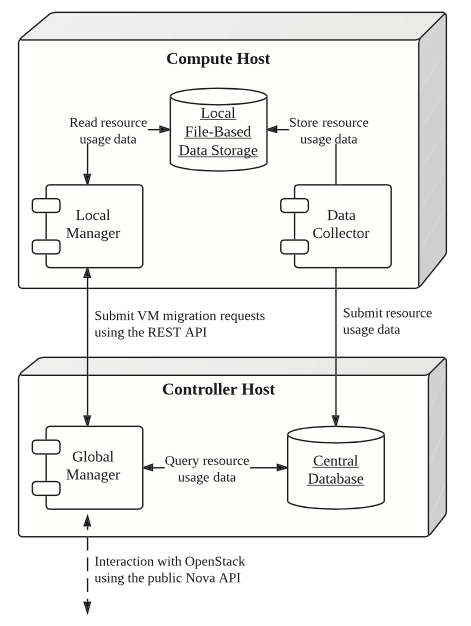
\includegraphics[width=\textwidth]{images/neat_arch.png}}
\label{fig:neat_arch}
\caption{The OpenStack Neat architecture \cite{beloglazov2014openstack}}
\end{figure}

Figure \ref{fig:neat_arch}~\cite[p.~7]{beloglazov2014openstack} represents the architecture of OpenStack Neat: it is mainly composed by a \textit{Global Manager} installed on the Controller node, and by a \textit{Local Manager} and a \textit{Data Collector} installed on every Compute node. The \textit{Global Manager} is responsible for making global management decisions such as mapping Virtual Machine instances to hosts, and initiating Virtual Machines live migrations; the \textit{Local Manager} makes local decisions such as deciding that the host is underloaded or overloaded and selecting Virtual Machines to migrate to other hosts; lastly the \textit{Data Collector} is responsible for collecting Virtual Machines and hypervisors resource usage data and for then storing the data locally and submitting it to the central database, which can also be distributed.\\
One of the main characteristics of OpenStack Neat is that it is designed to be distributed and external to OpenStack, in fact it acts independently of the base OpenStack platform and applies Virtual Machines consolidation by invoking OpenStack's public APIs. For that reason it has to be installed separately from OpenStack, following the limited instructions present on the GitHub page of the project\footnote{\url{github.com/beloglazov/openstack-neat}} and can not take advantage of tools like DevStack (see \ref{chap:openstack_devstack} on page \pageref{chap:openstack_devstack}) that automates the deploy and configuration of an OpenStack installation. \\


% -------------------------------------------------------------------------- %
% ------------------------- CLOUD TEST ENVIRONMENT ------------------------- %
% -------------------------------------------------------------------------- %

\section{Cloud test environments}
\label{sec:sota_test_env}

When provisioning a cloud we need to be able to test different environment configurations and algorithms, to analyze the behavior of new code that need to integrate with the environment, and to benchmark and collect data for research and experimentations. Unfortunately it can be expensive and complex to create and manage a cloud test environment in terms of time, resources and expertises, especially if the hardware resources like server machines or network infrastructures are limited. Fully understanding and handling an OpenStack installation is not easy, especially for non sysadmins like developers or researchers; it has a high learning curve and often a lot of time is needed to achieve the desired results.\\
There are some tools that reduce the impact of these complications are and make the process of setting up a cloud infrastructure experimentation environment easier and more manageable.
The growing need of advanced system management have made configuration management tools, such as Chef and Puppet, have become increasingly mainstream. These tools provide domain-specific declarative languages for writing complex system configurations, allowing developers to specify concepts such as ``what software packages need to be installed'', ``what services should be running on each hardware node'', etc. More recently OpenStack has started collaborating both with Chef (see section \ref{sub:sota_chef}) and Puppet (see section \ref{sub:sota_puppet}) to create new means to configure and deploy fully-functional OpenStack environments on bare-metal hardware, as well as on Vagrant virtual machines. The combination of a system management tool, like Chef or Puppet, and Vagrant can be used to setup a virtualized experimentation environment. However, these are complex sysadmin tools that require strong technical skills.\\
Below we present them and highlight their main features, as well as their strengths and weaknesses with respect to the topic of our thesis.

\subsection{Vagrant}
\label{sub:sota_vagrant}
Vagrant\footnote{\url{www.vagrantup.com}} is a virtualization framework for creating, configuring and managing development environments, written in Ruby. It is a wrapper around virtualization software such as VirtualBox, KVM, VMware and could be used together with configuration management tools such as Chef and Puppet.
Thanks to an online repository \footnote{\url{www.vagrantcloud.com}} it is possible to automatically download a Vagrant Box and run it with a single command: \code{vagrant up vagrant-box-name}.
It is also possible to create and configure custom Vagrant Box by simply writing a \code{Vagrantfile}:
\begin{lstlisting}[
  language=Ruby,
  numbers=none,
  caption={\texttt{Vagrantfile} example},
  label={lst:vagrantfile_example},
  ]
box      = 'trusty64'
url      = 'http://files.vagrantup.com/precise32.box'
hostname = 'customtrustybox'
domain   = 'example.com'
ip       = '192.168.0.42'
ram      = '2048'

Vagrant::Config.run do |config|
  config.vm.box = box
  config.vm.box_url = url
  config.vm.host_name = hostname + '.' + domain
  config.vm.network :hostonly, ip

  config.vm.customize [
    'modifyvm', :id,
    '--name', hostname,
    '--memory', ram
  ]
end
\end{lstlisting}
Provisioners in Vagrant allows one to automatically install and configure software in a Vagrant Box as part of the \code{vagrant up} process. Therefore it is easier to start with a base Vagrant Box, adapt it to your needs and eventually share it with other developers who can reproduce the same virtual development environment.\\
Vagrant is used together with configuration management software such as Chef and Puppet to create repeatable and easy to setup development and test environments that rely on Virtual Machines.


% ---------------------------------- CHEF ---------------------------------- %

\subsection{Chef}
\label{sub:sota_chef}

\subparagraph{Description}
\label{subp:sota_chef_desc}

Chef\footnote{\url{www.chef.io}} is a configuration management tool used to streamline the task of configuring and maintaining servers in a cloud environment. It can be integrated with cloud-based platforms such as Rackspace, Amazon EC2, Google Cloud Platform, OpenStack and others. It is written in Ruby and Erlang and uses a domain-specific language (DSL)\footnote{A programming language specialized to a particular application domain.} for writing configuration files called \textit{recipes}. \textit{Recipes} are used to define the state of certain resources\footnote{A resource state is a combination of installed software, running services, and configurations.}, and everything that is required to configure the different parts of the system. They state what software should be installed (together with any required dependencies), services that should be run or files that should be written. Given a \textit{recipe} Chef ensures that all the software is installed in the right order and that each resource state is reached, eventually correcting those resources in a undesired state; \textit{recipes} can be collected into \textit{cookbooks} to be more maintainable and powerful. In addition Chef offers a centralized hub, called Chef Supermarket\footnote{\url{supermarket.chef.io}}; it collects a large number of \textit{cookbooks} from the community that are freely downloadable.\\
A base installation of Chef comprises three main components: a \code{chef-server} that orchestrates all the Chef processes, multiple \code{chef-clients} found on all the servers, and the user workstation that communicates with the Chef Server to launch commands.\\
To simplify communication with the \code{chef-server} Chef provides a command-line tool called Knife that helps users manage nodes, \textit{cookbooks} and \textit{recipes}.

\subparagraph{Chef and OpenStack}
\label{subp:sota_chef_openstack}

Chef and OpenStack can be combined and used together in different ways, many of which have a different goal compared to our thesis. It is possible, in fact, to deploy and manage a production OpenStack installation running on multiple servers and supervised by a Chef Server (using the subcommand \code{knife openstack}) to control the OpenStack APIs through Chef and to instantiate new physical servers with a \code{chef-client} or turn some off (\code{knife openstack server create / delete}).
In this situation you can achieve a ``1 + N'' OpenStack configuration. In this case the OpenStack services are predefined and you cannot configure an ad hoc configuration.
It is also possible to have an ``All-in-One'' configuration, where all the OpenStack services are installed on a single node.\\
These configurations can be achieved with the help of Vagrant that will cover all the steps to install OpenStack on a virtual machine and configure all its services (excluded Block Storage, Object Storage, Metering, and Orchestration). Within the OpenStack chef-repo\footnote{\url{https://github.com/stackforge/openstack-chef-repo}} there is a \textit{recipe} to configure a VirtualBox virtual machine that will host and All-in-One installation. Here is a part of it:

\begin{lstlisting}[
  float,
  language=Ruby,
  numbers=none,
  caption={Recipe to run an ``All-in-One'' configuration (\texttt{aio-nova.rb})},
  label={lst:aio_recipe},
  ]
machine 'controller' do
  add_machine_options vagrant_config: controller_config
  role 'allinone-compute'
  role 'os-image-upload'

  chef_environment 'vagrant-aio-nova'
  file('/etc/chef/openstack_data_bag_secret',
       "#{File.dirname(__FILE__)}/.chef/encrypted_data_bag_secret")
  converge true
\end{lstlisting}

Of course it is possible to setup a ``1 + N'' configuration using different \code{Vagrantfiles} to create and configure one VM for the Controller and N VMs for the Compute nodes. However it is unlikely to succeed in running a lot of VMs on the same host, especially if they contain a fully functional OpenStack installation, since a Virtual Machine typically requires a significant amount of resources to operate.

\subparagraph{Pro and Cons}
\label{subp:sota_chef_pro_cons}

Chef is a very powerful tool to create, manage and configure cloud environments, and it offers a lot of functionalities to structure the desired architecture. In combination with Vagrant can also be used to setup test environments for development or research purposes.\\
However, with regard to this last aspect, it has several limitations:
\begin{itemize}
\item \textit{Performance}: because VMs are very resource greedy it is very difficult to achieve a ``1 + N'' configuration for development or research purpose on a single machine. On the other hand the ``All-in-One Compute'' solution that allows a full OpenStack installation on a single Virtual Machine is very simplistic and doesn't represent a real environment setting.
\item \textit{Lack of customization}: at the state of the art all of the described solutions install both the Controller node and the Compute node with a predefined set of installed services (in practice all the OpenStack service excluded Object Storage, Metering, and Orchestration are installed) so it is not possible to setup the environment with more or less services or new ones. In our case, in fact, we need to be able to decide which OpenStack services to install (for example we don't install OpenStack Network as a Service module, \code{Neutron}), as well as to implement a new one and install it (see chapter \ref{chap:consolidator} regarding our Consolidator service).
\item \todo{think others\dots}
\end{itemize}


% ---------------------------------- PUPPET ---------------------------------- %


\subsection{Puppet}
\label{sub:sota_puppet}

\subparagraph{Description}
\label{subp:sota_puppet_desc}

Similarly to Chef (described in section~\ref{sub:sota_chef}) Puppet\footnote{\url{www.puppetlabs.com}} is a configuration management system that allows you to define the state of a cloud infrastructure, which it will then automatically enforce.\\
Puppet uses a declarative model where one defines the resource states; its manifest files are written in a Ruby-like DSL. Configuration files are enclosed in \textit{modules}, self-contained bundles of code and data that are easy to share and reuse. There are a large amount of them on the Puppet Forge\footnote{\url{forge.puppetlabs.com}} repository.\\
Puppet is structured in a master-slave architecture: the master serves the manifests and the files, and the clients polls the master at specific intervals of time to get their configurations so that the master never pushes nothing to them.


\subparagraph{Puppet and OpenStack}
\label{subp:sota_puppet_openstack}

As seen for Chef, Puppet can be very useful when dealing with OpenStack installation and maintenance. To configure and deploy an OpenStack infrastructure with the help of Puppet one can download appropriate \textit{modules} from Puppet Forge; this simplifies most of the operations such as OpenStack instances provisioning, configuration management and others.
The module is \code{puppetlabs-openstack}\footnote{\url{github.com/puppetlabs/puppetlabs-openstack}}; using this module it is possible to deploy both a multi-node and an all-in-one installation. Compared to Chef, Puppet is a bit more flexible because it allows you to control more details about the OpenStack services that are to be installed on every node; for example, you can use the following instructions in the Puppet's manifest file of a node to achieve different results:

\textit{Controller node:}
\begin{lstlisting}[
  language=Ruby,
  numbers=none,
  caption={Portion of a manifest file for a controller node},
  label={lst:manifest_controller},
  ]
node 'control.localdomain' {
  include ::openstack::role::controller
}
\end{lstlisting}

\textit{Controller node:}
\begin{lstlisting}[
  language=Ruby,
  numbers=none,
  caption={Portion of a manifest file for a compute node},
  label={lst:manifest_compute},
  ]
node 'storage.localdomain' {
  include ::openstack::role::storage
}

node 'network.localdomain' {
  include ::openstack::role::network
}

node /compute[0-9]+.localdomain/ {
  include ::openstack::role::compute
}
\end{lstlisting}

Obviously, it is possible to configure multiple nodes to run in multiple Virtual Machines that are configured and launched with Vagrant and deploy the various OpenStack components with \code{puppetlabs-openstack}. This solution, is clearly difficult to achieve on a machine with a limited amount of resources; however also on a more powerful server machine this solution it is slightly feasible and scalable.

\subparagraph{Pro and Cons}
\label{subp:sota_puppet_pro_cons}
Puppet is an extremely powerful and mature tools for automated cloud infrastructure deploying: it streamlines the entire process and automates every step of the software delivery process.\\
However from our point of view we are more interested in knowing how it behaves when a single developer or a researcher needs to deploy a cloud infrastructure on a single machine with limited amounts of resources (a development workstation for example) and he/she has little sysadmin skills. With regard to this aspect Puppet used with Vagrant has some key limitations:

\begin{itemize}
\item \textit{Performance}: A single Virtual Machine generally need a remarkable amount of resources, especially to host an OpenStack installation; for this reason it is very unlikely that one will be able to run on a single machine the number of Virtual Machines needed to deploy a realistic multi-node installation of OpenStack. Once again ``all-in-one'' solution is not sufficiently realistic, especially when testing algorithms or portions of code that involve multiple nodes.
\item \todo{think others\dots}
\end{itemize}

% ---------------------------------- CHEF ---------------------------------- %

\subsection{Docker}
\label{sub:sota_docker}
Docker\footnote{\url{www.docker.com}} is an open platform for developers and sysadmins to build, ship, and run distributed applications. Its core is the Docker Engine: it exploits Linux containers to virtualize a guest Operating System on a host avoiding the considerable amount of resources necessary to run Virtual Machines.\\
The main difference between the Docker solution and Virtual Machines solution lie in the way in which the hypervisor and the Docker Engine manage the guest Operating System. A Virtual Machine, as shown in figure ~\ref{fig:docker_vm} on page~\pageref{fig:docker_vm}, hosts a complete Operating System including application, dependency libraries, and, more important, the kernel; the Docker Engine, on the other hand, runs as an isolated process in userspace on the host operating system and allows all the guest containers to share the kernel. Thus, it enjoys the resource isolation and allocation benefits of Virtual Machines, but is much more portable and efficient; for our goals this aspect allows us to run at the same time a larger number of containers compared to what we are able to achieve with Virtual Machines and also to ship pre-built images of our modules.\\
To configure and build a container image you have to write a Dockerfile, that is a text document containing all the commands which you would have normally executed manually in order to take the container to the desired state, and then call \code{\$ sudo docker build .} from the directory containing the file. The command \code{\$ sudo docker run} will finally launch the container.\\
Docker offers an online platform called Docker Hub\footnote{\url{hub.docker.com}} where you can upload both Dockerfile and pre-built container images to streamline the sharing process.
    
\begin{figure}[!ht]
\centering{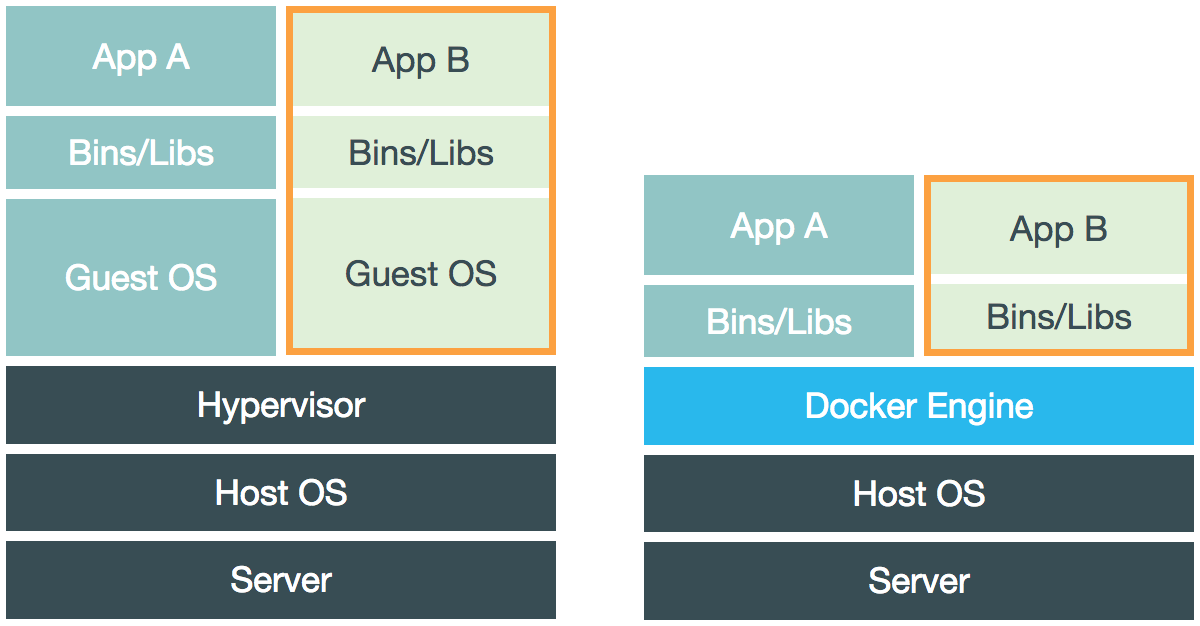
\includegraphics[width=\textwidth]{images/docker_vs_vm.png}}
\label{fig:docker_vm}
\caption{Hypervisor and Docker Engine}
\end{figure}

% ------------------------------- DOCKENSTACK ------------------------------- %

\subsection{Dockenstack}
\label{sub:sota_dockenstack}
One of the first attempts to create a cloud test environment based on OpenStack and Docker is Dockenstack\footnote{\url{github.com/ewindisch/dockenstack}}. It is an independent and not actively supported project, but is a good starting point to show the potential derived from using Docker.\\
The project is basically composed of a Dockerfile and a bunch of scripts that will setup and configure an OpenStack installation using DevStack (\todo{shall we talk about it in the intro?}) in a Docker container.\todo{cmd spiegare}\\
A pre-built image is available on Docker Hub, so with the command \code{docker run -privileged -t -i ewindisch/dockenstack} Docker will automatically download and run the container.\\
This made it a good solution for beginners wanting to learn OpenStack, but inadequate for advanced experiments, such as experiments regarding Virtual Machine placement and server consolidation algorithms.



%--------------------------------------------------------------------------------
% aDock
%--------------------------------------------------------------------------------
\chapter{aDock}
\label{chap:adock}
%!TEX root = ../thesis.tex
%%--------------------------------------------------------------------------
%% ADOCK
%%--------------------------------------------------------------------------

%% REMEMBER:
%% - section
% \section{Section Title}
% \label{sec:section_title}
%
% - subsection
% \subsection{Subsection Title}
% \label{sub:sub_title}
%
% - paragraph
% \subparagraph{Paragraph Title}
% \label{subp:subp_title}


% --------------------------------------------------------------------------- %
% ---------------------------------- ADOCK ---------------------------------- %
% --------------------------------------------------------------------------- %


\section{Our Solution, aDock}
\label{sec:adock_intro}
The lack of a uniform and standardized test environment for cloud systems brought us to develop aDock.\\
aDock is a suite of tools that lets the final user deploy a complete OpenStack system; run simulations against it; collect output data and view results on a friendly user interface.\\
We chose OpenStack as cloud computing software platform, because of its open-source nature and because of its continuous evolution with the aim of keeping up with the last cloud standards.\\
Our intended users are OpenStack developers who need to run their code in a fully functional environment and researchers who want to try their algorithm on a complete cloud system to test out its behavior.

\section{Requirements}
\label{sec:adock_reqs}
In this section, we will identify both functional and non-functional requirements for aDock.

\subsection{Functional Requirements}
\label{sub:func_req}

\paragraph{FR1}\label{p:fr1} \emph{aDock should provide tools to deploy a complete environment.} \hfill \\
A user should be able to start and update OpenStack's nodes with a single command. aDock should provide the user with an abstraction of a server called ``node''. The ``node'', in its depth, is an Ubuntu based Docker container, shipped with OpenStack services dependencies. A user should be able to decide which services will be installed and started on each node and their internal configuration using a configuration file.
\subparagraph{Solution} FakeStack (see section \ref{sec:fakestack}) is the aDock module which provides the user with the specified tools. Starting a node is as easy as \code{\$ run\_node}. A node can be configured by means of a simple configuration file. Nodes are of two types, \textit{controllers} and \textit{computes}. Controller nodes are different from compute ones because they are shipped with \textit{MySQL} and \textit{RabbitMQ} installations.

\paragraph{FR2}\label{p:fr2} \emph{aDock should provide a tool to run simulations.} \hfill \\
If the user puts his/her code into OpenStack he/she probably aims at running simulations and examine the new piece of code behavior in interacting with the entire system. Simulations should be configurable according to the user needs and repeatable.
\subparagraph{Solution} Oscard (see section \ref{sec:oscard}) is the aDock module which takes care of running repeatable and configurable simulations against an OpenStack system.

\paragraph{FR3}\label{p:fr3} \emph{aDock should persistently store simulations output.} \hfill \\
Once a simulation has been run, it could be interesting to store the outputs of it in terms of generic metrics about the system, such as the average of the number of compute nodes active during the simulation, the average of virtual CPUs used and so on.
\subparagraph{Solution} Oscard, by default, stores the aggregates of a simulation into a Firebase\footnote{\url{https://www.firebase.com/}} backend. In our case, the backend is called Bifrost (see section \ref{sec:others}).

\paragraph{FR4}\label{p:fr4} \emph{aDock should provide a user interface} \hfill \\
Although Firebase provides an interactive user interface, data is displayed in a \textit{JSON} fashion and it is, therefore, not easily understandable and browseable. Simulations results should be displayed to user in a friendly manner, using charts to give the user a glimpse of the current situation. Data representation should be given in real-time.
\subparagraph{Solution} Polyphemus (see section \ref{sec:others}) is the aDock module which takes care of displaying to the user real-time simulation results in a friendly manner.

\subsection{aDock Architecture}
\label{sub:adock_arch}
aDock turns out to be a modular system where each component is configurable and has a precise purpose. FakeStack is employed to start nodes; Oscard runs simulations and collects aggregates on Bifrost; Polyphemus is the eye on the data that shows the user the results obtained.
In figure~\ref{fig:adock_arch} we highlight the general architecture of aDock.

\todo{insert aDock architecture picture}

\subsection{Non-Functional Requirements}
\label{sub:nonfunc_req}
As opposed to functional requirements, aDock has very strong non-functional requirements in order to give a suitable testing environment to our stakeholders. In general we take leverage of Docker and DevStack and use their biggest strength. Docker gives us high speed in running containers and sandboxing by construction and makes aDock cross-platform; while DevStack gives us great flexibility and configurability for what concerns OpenStack services.

\paragraph{NFR1}\label{p:nfr1} \emph{Users should be able to choose which code is running in OpenStack.} \hfill \\
Before booting the entire system the user should be able to choose if he/she wants to run OpenStack code from a precise code repository which is, in general, the better and more supported way to version and share code among developers and even physical machines. Speaking in Git\footnote{\url{http://git-scm.com/}} terms, a user could choose to run the most up to date code (which may be buggy) and so get the code from branch \code{master}, or maybe get a much more stable OpenStack version and get the code from branch \code{stable/juno}. The most interesting fact (and this is the scenario we have in our mind) is that the user could choose to fork an OpenStack service and see his/her code running onto nodes.

\subparagraph{Solution} All of this is achievable thanks to DevStack, which installs OpenStack services cloning repositories from GitHub and running \code{python setup.py install}. By default, DevStack clones official OpenStack repositories from branch \code{master}, but it is possible to specify different repository URLs and branches for each of the OpenStack services by means of \code{local.conf} files.

\paragraph{NFR2}\label{p:nfr2} \emph{aDock should be lightweight.} \hfill \\
Users often need to test algorithms that, by design, target the management and/or optimization of tens of physical servers. Since we can assume that not everyone will have that amount of resources, we believe that aDock should be as light-weight as possible. It should be possible to run aDock on limited hardware, potentially even on one's personal laptop. It is under this assumption that sandboxing becomes important; indeed, the experimentation environment should not have any sort of repercussions on the user's machine; we want the user to be able to build and tear down the environment with no consequences.

\subparagraph{Solution} Docker is a virtualization system which relies on Docker containers which are much more lightweight than virtual machines\footnote{\url{http://devops.com/blogs/devops-toolbox/docker-vs-vms/}} \todo{is the ref authoritative?}. Docker gives us, by construction, speed and lightness.

\paragraph{NFR3}\label{p:nfr3} \emph{The experimentation environment should be highly configurable.} \hfill \\
Our primary goal with aDock is to provide a fast and easy way to create the experimentation environment. We believe that building a system which allows users to design the overall architecture of the cloud system is out of scope of this thesis, mainly because of the intrinsic high complexity and vastness of OpenStack's system itself. Up to now, as a proof of concept, we will focus on ``1 + N'' architecture, with $1$ controller node and $N$ compute nodes.

\subparagraph{Solution} The possibility to configure the system still remains in configuring OpenStack services in terms of their internal behavior. This is achieved, again, thanks to DevStack, which allows us to configure OpenStack in all its aspects through \code{local.conf} file. Each service can be configured in each of DevStack installation phases. Each service, during installation, passes through \textbf{local}, \textbf{pre-install}, \textbf{install}, \textbf{post-config}, \textbf{extra} phases\footnote{\url{http://docs.openstack.org/developer/devstack/configuration.html\#local-conf}}. Configuring a service is as simple as adding few lines to \code{local.conf} file:

\begin{lstlisting}[title=Adding per-service configuration to DevStack's local.conf file]
[[post-config|\$NOVA-CONF]]
[DEFAULT]
verbose=True
logdir=/var/log/my-nova-logdir

# SCHEDULER
compute_scheduler_driver=nova.scheduler.MyMagicScheduler
# VIRT DRIVER
compute_driver=nova.virt.fake.MyAmazingFakeDriver
\end{lstlisting}


\paragraph{NFR4}\label{p:nfr4} \emph{aDock should allow users to run repeatable simulations.} \hfill \\
It is of paramount importance that users be able to compare their results with baseline approaches, as well as with related work from the state of the art. aDock should make it easy to compare an experiment's results with those of others on the same simulations.

\subparagraph{Solution} Oscard will take into account repeatability both giving the possibility to run the same simulation, at the same time, on multiple hosts, both using pseudo-randomization (see section \ref{sec:oscard}).

% --------------------------------------------------------------------------- %
% -------------------------------- FAKESTACK -------------------------------- %
% --------------------------------------------------------------------------- %

\section{FakeStack}
\label{sec:fakestack}

% --------------------------------------------------------------------------- %
% ---------------------------------- OSCARD --------------------------------- %
% --------------------------------------------------------------------------- %

\section{Oscard}
\label{sec:oscard}

% --------------------------------------------------------------------------- %
% --------------------------- BIFROST + POLYPHEMUS -------------------------- %
% --------------------------------------------------------------------------- %

\section{Other Components}
\label{sec:others}

%--------------------------------------------------------------------------------
% Consolidator
%--------------------------------------------------------------------------------
\chapter{Nova Consolidator}
\label{chap:consolidator}
%!TEX root = ../thesis.tex
%%--------------------------------------------------------------------------
%% NOVA CONSOLIDATOR
%%--------------------------------------------------------------------------
OpenStack already performs virtual machine placement. This is accomplished thanks to its \texttt{nova-scheduler} service. Once a virtual machine is created (or, in certain cases, resized or live migrated) the scheduler decides which of the available compute nodes can host\footnote{The policies by which a node can host or not a virtual machine are defined by the precise filter which scheduler has been equipped with.} the virtual machine (this phase is called \textit{filtering}) and then selects the best\footnote{Again, it depends on which weighter is used.} among them (this phase is called \textit{weighting}).

OpenStack \emph{doesn't} perform virtual machine consolidation. Each of the operations on virtual machines are issued by the user that owns them (or by \texttt{Heat} for him/her).

Virtual machine consolidation is a technique by which virtual machines locations on hosts are changed to achieve a better resource utilization in the whole system. Thus, virtual machines are periodically live (or cold) migrated to other hosts if some policy determines that its place is the wrong in that precise moment. The policy adopted is determined by the \emph{consolidation algorithm} used.

To add virtual machine consolidation feature to OpenStack we added a service to \texttt{Nova} called \texttt{nova-consolidator}. The new service is implemented in module \code{nova.consolidator} which provides a \code{nova.consolidator.base.BaseConsolidator} class which can be extended to write custom consolidators (see section \ref{sec:cons_base}) and some consolidation algorithms, both custom and taken from the state of the art (see section \ref{sec:cons_algs}).

\section{Consolidator Base}
\label{sec:cons_base}

Almost every service into OpenStack has three main components, the \emph{command}\footnote{In our case, \code{nova.cmd.consolidator}.} (its function \code{main} will be executed at service startup\footnote{When DevStack runs \code{python setup.py install}, \textit{PyPI} generates an executable file placed at \texttt{/usr/local/bin} called \texttt{nova-consolidator} (see note \ref{note:pypi}). It is necessary to make DevStack aware of the new service created to make it install and start it. As a result we had to fork DevStack repository and edit the function \code{start\_nova\_rest} in \texttt{/lib/nova} (see \url{https://github.com/affear/devstack/blob/n-cons/lib/nova}).}); the \emph{manager}\footnote{In our case, \code{nova.consolidator.manager}.}, which contains the real logic of the service and the \emph{RPC\footnote{Remote Procedure Call} API}\footnote{In our case, \code{nova.consolidator.rpcapi}}, which is used among OpenStack services to communicate\footnote{\url{https://github.com/affear/nova/tree/n-cons/nova/consolidator}}.

The command basically instantiates a \code{nova.service.Service} object with name ``\texttt{nova-consolidator}''. The service, in turn, instantiates a \code{nova.consolidator.manager.ConsolidatorManager} object; starts its RPC server and its \emph{periodic tasks}. As we can see in listing \ref{lst:cons_manager}\footnote{\label{note:cons_code}The code has been properly cut to fit the page and the reader needs.}, \code{ConsolidatorManager} exposes only one periodic task which is \code{consolidate} method.
Its period is defined in \texttt{/etc/nova/nova.conf} file (which can be edited using DevStack. See ~\ref{sub:fakestack_conf}) in option \texttt{consolidation\_interval} as well as the consolidator class used by the manager. When the manager is created a consolidator object is obtained using the \texttt{consolidator\_class} provided. Then, periodically, \code{consolidate} task is invoked. \code{consolidate} function \emph{delegates} consolidation to the consolidator object obtaining the necessary migrations to be performed. Once migrations are obtained, they are applied using \texttt{nova-compute}'s API.

The consolidator class is, by default, \code{nova.consolidator.base.BaseConsolidator} (see listing \ref{lst:cons_base}\footnoteref{note:cons_code}), which does nothing but defining a base class to be extended with real consolidation algorithms. Its \code{get\_migrations} method, in fact, returns an empty list of migrations. The most important method in \code{BaseConsolidator} is \code{consolidate}, which is the method the manager delegates consolidation to.

This method creates a snapshot of the system (see \ref{sub:cons_obj}) and passes it to \code{get\_migrations} method. \code{get\_migrations} will implement the consolidation algorithm desired. Eventually, a transitive closure on migrations is applied\footnote{If instance $I$ is moved first to host $A$ and then to host $B$; instance $I$ is only moved to host $B$.} and the migrations are returned to the manager.

\begin{lstlisting}[
	float,
	language=python,
	caption={Code for \texttt{nova.consolidator.manager.ConsolidatorManager}},
	label={lst:cons_manager},
	tabsize=2
]
class ConsolidatorManager(manager.Manager):

	def __init__(self, *args, **kwargs):
		self.compute_api = compute_api.API()
		self.consolidator = importutils.\
			import_class(CONF.consolidator_class)()
		# lines skipped

	@periodic_task.\
		periodic_task(spacing=CONF.consolidation_interval)
	def consolidate(self, ctxt):
		migrations = self.consolidator.consolidate(ctxt)
		for m in migrations:
			self._do_live_migrate(ctxt, m)

	def _do_live_migrate(self, ctxt, migration):
		instance = migration.instance
		host_name = migration.host.host
		# exception catching skipped
		self.compute_api.live_migrate(
			ctxt, instance,
			False, False, host_name
		)
\end{lstlisting}

\begin{lstlisting}[
	float,
	language=python,
	caption={Code for \texttt{nova.consolidator.base.BaseConsolidator}},
	label={lst:cons_base},
	tabsize=2
]
class BaseConsolidator(object):

	class Migration(object):
		def __init__(self, instance, host):
			super(BaseConsolidator.Migration, self).__init__()
			self.instance = instance
			self.host = host

	# _transitive_closure method
	# implementation skipped

	def consolidate(self, ctxt):
		snapshot = Snapshot(ctxt)
		migs = self.get_migrations(snapshot)
		return self._transitive_closure(migs)

	def get_migrations(self, snapshot):
		return []
\end{lstlisting}

\subsection{Objects}
\label{sub:cons_obj}
We thought that it wouldn't have been fair to leave to the user the duty to learn and understand OpenStack's complex database APIs.
Due to this fact, we developed \code{nova.consolidator.objects}, which is a module that defines an abstraction of system snapshot to be used in method \code{get\_migrations} by developers. The module provides the class \code{nova.consolidator.objects.Snapshot}. A \code{Snapshot} object offers attributes to access all information about the system, such as current active nodes and instances both for each node and, generally, in the system itself. The \code{Snapshot} is thought to be renewed at each consolidation cycle. So, any attribute is lazily obtained on its first call: subsequent invocations of that attribute won't refresh snapshot's state. The Snapshot is, thus, entirely cached\footnote{Once an instance or a compute node is obtained it will not be queried again on OpenStack's database. Its status is \emph{frozen} at the moment the first query has been performed. To refresh a \code{Snapshot} it is necessary to create a new \code{Snapshot} object.}.

In detail, a \code{Snapshot} object offers active nodes (\code{nodes} attribute) and all, running, migratable\footnote{According to us, an instance is \emph{migratable} when its state is \texttt{ACTIVE} and its power state id \texttt{RUNNING}.} and not instances. Instances are \code{nova.objects.instance.Instance}\footnote{\url{https://github.com/openstack/nova/blob/master/nova/objects/instance.py}} objects; nodes are wrappers for \code{nova.objects.compute\_node.ComputeNode}\footnote{\url{https://github.com/openstack/nova/blob/master/nova/objects/compute_node.py}} objects, which add the possibility to get all, running, migratable and not instances per compute node.

In any case, the developer is not thought to instantiate \code{Snapshot} objects, because this is up to \code{consolidate} method, which already instantiates and passes the current system snapshot to method \code{get\_migrations}, which is the \emph{only} method which needs to be overridden by the user in a custom consolidator class.

In listing \ref{lst:cons_snapshot} we provide an example of using a \code{Snapshot} in a python script.

\begin{lstlisting}[
	float,
	language=python,
	caption={An example of using a \texttt{Snapshot} object},
	label={lst:cons_snapshot},
	tabsize=2
]
from nova import config, objects, context
from nova.consolidator.objects import Snapshot

# Init operations
config.parse_args('')
objects.register_all()
ctxt = context.get_admin_context()

# Using the Snapshot
s = Snapshot(ctxt)
nodes = snapshot.nodes # all compute nodes
node = nodes[0] # the first node
instances = node.instances # all instances on that node (list)
print node.vcpu
print node.id
print instances[0].flavor
# `node` has all attributes as
# nova.objects.compute_node.ComputeNode has,
# as well as `instances[0]` has all attributes as
# nova.objects.instance.Instance has.

nodes_new = snapshot.nodes
# nodes are not refreshed because they are cached!
assert nodes == nodes_new # evaluates to True
\end{lstlisting}

\section{Algorithms}
\label{sec:cons_algs}
In this section, we explain in detail consolidation algorithms that we implemented in our \texttt{nova-consolidator}. Each of the algorithms proposed is run inside a consolidator class that inherits from \code{nova.consolidator.base.BaseConsolidator}, inside \code{get\_migrations} method.

\subsection{Random Algorithm}
\label{sub:algs_rnd}
The first algorithm we implemented is the random one\footnote{\url{https://github.com/affear/nova/blob/n-cons/nova/consolidator/base.py}}. This algorithm was implemented for testing purpose and to see if even randomization could bring improvement in resource optimization, given that virtual machines are never moved in OpenStack\footnote{Except for when a user decides to, or on a resize call. When a virtual machine is resized to a flavor which is too big for the current host, it is migrated to a suitable one.}.

The algorithm takes, by configuration, a percentage of migratable instances to be migrated to other compute nodes. Instances are randomly chosen from hosts and their destination is randomly chosen among remaining hosts. Choices are not taken taking into account host suitability. The algorithm by itself doesn't rely on the fact that migrations will be applied. If a migration fails, due to resource usage problems, it is not a problem.

Random algorithm is highlighted in in listing \ref{lst:rnd_alg}\footnoteref{note:cons_code}.

\begin{lstlisting}[
	float,
	language=python,
	caption={Code for random algorithm},
	label={lst:rnd_alg},
	tabsize=2
]
def get_migrations(self, snapshot):
	nodes = snapshot.nodes
	no_nodes = len(nodes)
	migration_percentage = float(CONF.consolidator.migration_percentage) / 100
	no_inst = len(snapshot.instances_migrable)
	no_inst_migrate = int(no_inst * migration_percentage)

	# if no_inst_migrate == 0
	# or no_nodes < 2, then
	# return empty list.
	# Cannot migrate.

	migs = []
	while no_inst_migrate > 0:
		nodes_cpy = list(nodes) # copy nodes list

		from_host = choose_host(nodes_cpy)
		# choose_host code is skipped.
		# The chosen node is randomly chosen
		# taking into account that it has to host
		# at least one instance.

		inst_on_host = from_host.instances_migrable
		no_inst_on_host = len(inst_on_host)

		top_bound = min(no_inst_on_host, no_inst_migrate)
		n = random.randint(1, top_bound)
		no_inst_migrate -= n

		instances = random.sample(inst_on_host, n)
		nodes_cpy.remove(from_host) # do not choose same host
		to_host = random.choice(nodes_cpy)
		for i in instances:
			migs.append(self.Migration(i, to_host))

	return migs
\end{lstlisting}

\subsection{Genetic Algorithm}
\label{sub:algs_ga}
The idea to use a genetic algorithm to solve virtual machine consolidation problem is taken from the state of the art (see section \ref{sec:sota_ga}), although heavily revisited from us\footnote{https://github.com/affear/nova/tree/n-cons/nova/consolidator/ga}.

Our genetic algorithm uses a list as chromosome structure. Each element of the list (a gene) is considered as a migratable instance an its value is the hostname of the compute node that will host the instance. At first, we developed the algorithm as a ``standard'' genetic algorithm. So, it provided a crossover step. After some simulation we realized that $100\%$ of the children generated were unhealthy\footnote{A child is considered unhealthy when it violates system constraints. For example, instances on a node exceed its memory capacity.}. Suddenly, we realized that the probability of generating a healthy child was close to zero because of the tightness of system constraints. Thus, the crossover step became useless and we decided to turn it into a massive mutation. While in crossover we chose\footnote{Chromosome are chosen among the whole population using a specific selection algorithm.} two chromosomes, father and mother, and crossed them; now we choose only one chromosome and massively\footnote{We change the value of an high percentage of its genes.} mutate it.

The algorithm is configurable in all of its aspects:
\begin{description}
	\item[prob\_mutation] (Defaults to $0.8$) The probability to apply mutation on a chromosome.
	\item[mutation\_perc] (Defaults to $10$) The percentage of the genes to be mutated in a chromosome, once mutation is decided to be applied.
	\item[selection\_algorithm] (Defaults to \code{nova.consolidator.ga.functions.RouletteSelection}) The selection algorithm used. Selection algorithm plays its role when its time to decide which chromosomes to cross (in our case, mutate) to generate a new children to add to the new population (an implementation of tournament selection is provided in \code{nova.consolidator.ga.functions.TournamentSelection}).
	\item[fitness\_function] (Defaults to \code{nova.consolidator.ga.functions.NoNodesFitnessFunction}) Fitness function is the one thats establishes how much the chromosome fits the solution wanted (see listing \ref{lst:ga_fitness} for \code{NoNodesFitnessFunction} implementation).
	\item[population\_size] (Defaults to $500$) The size of the population.
	\item[epoch\_limit] (Defaults to $100$) The number of epochs above what the algorithm stops.
	\item[elitism\_perc] (Defaults to $0$) The percentage of chromosomes that will pass to the next epoch. The number \texttt{N} of elite chromosomes is determined from this option and \texttt{population\_size} option. At each step the best \texttt{N} chromosomes (according to the fitness function used) will pass to the next epoch.
\end{description}

There is another option which is \texttt{best} (defaults to $False$). After running some simulation, we discovered that most of the epochs run without improving the fitness of the best chromosome and so we spent time in generating useless children. To overcome this problem we revisited mutation. Mutation is applied changing a gene's value and maintaining the chromosomes validity. To change a gene value means moving an instance to another compute node. The other compute node, normally, is chosen randomly among suitable nodes\footnote{Nodes that, hosting the machine, will not exceed their capacity in terms of vCPUs, memory and disk.}. When \texttt{best} is set to $True$, the other compute node is no more chosen randomly but as the best\footnote{The most busy compute node.} among suitable compute nodes. With this change in mutation logic, it turns out that the best chromosome generated in the very first epoch will almost never be exceeded by another one. Thus, this variant, truncates to number of epochs to $1$. The ``best'' variant is something vaguely similar to a genetic algorithm because there is no evolution except from selection logic and mutation.

In algorithm \ref{alg:ga} we provide a high-level pseudo-code for our genetic algorithm.

\begin{lstlisting}[
	float,
	language=python,
	caption={Code for \texttt{NoNodesFitnessFunction}},
	label={lst:ga_fitness},
	tabsize=2
]
class NoNodesFitnessFunction(FitnessFunction):
  # The higher the less nodes are used:
  #  - no_nodes = 1: fitness = 1
  #  - no_nodes -> infinite: fitness -> 0

  def get(self, chromosome):
    return float(1) / len(set(chromosome))
\end{lstlisting}

\begin{algorithm}[H]
\caption{Pseudo-code for our genetic algorithm}
\label{alg:ga}
\begin{algorithmic}[0]
	\State population = \texttt{population\_size} random generated valid chromosomes
	\State epoch\_count = 0
	\State

	\Procedure{new\_chromosome}{}\Comment{Returns a new chromosome}
		\State Select a chromosome from population using \texttt{selection\_algorithm}
		\State Mutate the chromosome with probability \texttt{mutation\_prob}
		\State Return the chromosome obtained
	\EndProcedure
	\State
	\Procedure{next}{}\Comment{Returns next population}
		\State Take the elite from current population (\texttt{elitism\_perc})
		\State Add it to new population
		\While{new population is not as big as \texttt{population\_size}}
			\State Add to new population the result of new\_chromosome procedure
		\EndWhile
	\EndProcedure
	\State

	\While{epoch\_count is less than \texttt{epoch\_limit}}
		\State population = next()
		\State Increment epoch\_count
	\EndWhile

	\State
	\State return population
\end{algorithmic}
\end{algorithm}

\subsection{Holistic Algorithm}
\label{sub:algs_holistic}
As well as genetic algorithm, holistic algorithm\footnote{\url{https://github.com/affear/nova/tree/n-cons/nova/consolidator/holistic}} is taken from the state of the art (see \ref{sec:sota_holistic}). In algorithm \ref{alg:holistic} we provide a high-level pseudo-code for holistic algorithm.

\begin{algorithm}[H]
\caption{Pseudo-code for holistic algorithm}
\label{alg:holistic}
\begin{algorithmic}[0]
	\State nodes = nodes from given snapshot
	\State no\_nodes = number of nodes given in snapshot
	\State new\_state = mappings (instance: node)
	\State
	\ForAll{node in nodes}
		\State node = least loaded node
		\State
		\If{node has no instances}
			\State continue
		\EndIf
		\State
		\State Sort node's migratable instances from biggest to smallest
		\State
		\ForAll{instance in node's instances}
			\State to\_node = most loaded node that can host instance
			\If{to\_node doesn't exist}
				\State continue
			\EndIf
			\State add mapping (instance: to\_node) to new\_state
		\EndFor
	\EndFor
	\State
	\State return new\_state
\end{algorithmic}
\end{algorithm}

%--------------------------------------------------------------------------------
% Evaluations
%--------------------------------------------------------------------------------
\chapter{Evaluation}
\label{chap:eval}
%!TEX root = ../thesis.tex
%%--------------------------------------------------------------------------
%% EVALUATION
%%--------------------------------------------------------------------------

Due to the two-topic nature of this thesis we split this chapter into two sections. Section \ref{sec:eval_adock} discusses about aDock system evaluation, while section \ref{sec:eval_cons} discusses about the evaluation of the different consolidation algorithms implemented by us into OpenStack.

\section{aDock}
\label{sec:eval_adock}
This section presents the results of the experiments we carried out to evaluate aDock's capability to create fully functional experimentation environments based on OpenStack, and its scalability.

The first experiments we show were performed on a Dell PowerEdge T320 server\footnote{Intel Xeon E5-2430 2.20GHz, 15M Cache, Ubuntu 14.04LTS 3.13.0-32-generic X86\_64. 16GB of RAM and SWAP. No SSD equipped.}. This is not a high-end server, and can be bought nowadays for less the one thousand euros. 

In the experiment we created an aDock environment with $1$ controller container and $1$ compute container. We then progressively increased the number of compute containers to identify how many could be run at the same time. Keep in mind that each container was actively running OpenStack code. The maximum number of compute nodes that can be run in a two-node architecture with legacy networking, before the controller becomes a management bottleneck, is $20$~\footnote{\url{https://docs.chef.io/openstack_architecture.html\#openstack-chef-single-controller-n-compute}}. Therefore, we wanted to see whether we could reach this threshold on a single machine, and to what extent we could surpass it. Table~\ref{tab:adock_server} shows the results of our experiments.

\begin{table}[h!]
\centering
  \begin{tabular}{| c | r | r | r | r |}
  \hline
  \textbf{Config} & \textbf{AvgTime [sec]} & \textbf{AvgCPU [\%]} & \textbf{AvgMem [\%]} & \textbf{AvgSwap [\%]}  \\
  \hline
  clean & 588 & 0.16 & 1.875 & 0 \\
  \hline
  1 + 0 & 188 & 2.295 & 30.956 & 0 \\
  \hline
  1 + 1 & 185 & 2.707 & 38.076 & 0 \\
  \hline
  1 + 6 & 182 & 5.616 & 65.979 & 0 \\
  \hline
  1 + 12 & 189 & 5.478 & 98.847 & 0.038 \\
  \hline
  1 + 22 & 191 & 5.54 & 98.869 & 0.257 \\
  \hline
  1 + 42 & 214 & 7.59 & 98.978 & 21.865 \\
  \hline
  \end{tabular}
  \vspace{2mm}
  \caption{aDock's performance on a PowerEdge T320 server.}
  \label{tab:adock_server}
\end{table}

As we can see we succeeded in reaching ``1 + 20'' architecture and overcome it to ``1 + 42''. We think this is a great result, because it could possibly allow the user to try different architectures with less compute nodes and more controller nodes. Although, up to now, aDock doesn't support architectures with more than one controller node by default.

On of our aims is to understand if a user can use aDock on his/her laptop without owning a server. So, we tried to deploy an aDock environment on two different laptops. We left Google Chrome\footnote{\url{https://www.google.it/chrome/browser/desktop/}} (our favorite web browser) and Sublime Text\footnote{\url{http://www.sublimetext.com/}} (our favorite text editor) running because we assumed that a user is developing and browsing while using aDock platform\footnote{Keep in mind that this fact impacts considerably the test. Google Chrome, for example, increases resource usage so much, that Google itself provides ways to lower it (see \url{https://support.google.com/chrome/answer/6152583?hl=en}).}.

Our goal was to deploy a ``1 + 5'' configuration (one controller node and five compute nodes), which we think it is a configuration which satisfies most of testing use cases. The test took place with the same form of the server one, except from the fact that we stopped at ``1 + 5'' architecture goal. In table \ref{tab:adock_ultra} we show the results of the experiment conducted on a Samsung SERIES 5 ULTRA\footnote{Intel Core i5 1.6 GHz, Linux Mint 3.13.0-24-generic XFCE, 4GB of RAM and SWAP. No SSD equipped.}, while in table \ref{tab:adock_macpro} we show results on an Apple MacBook Pro (Early 2011)\footnote{Intel Core i5 2.3 GHz, Mac Os X Yosemite, 8GB of RAM, SWAP is dynamically allocated. SSD equipped.}.

\begin{table}[h!]
\centering
  \begin{tabular}{| c | r | r | r | r |}
  \hline
  \textbf{Config} & \textbf{AvgTime [sec]} & \textbf{AvgCPU [\%]} & \textbf{AvgMem [\%]} & \textbf{AvgSwap [\%]}  \\
  \hline
  clean & 1736 & 12.34 & 52.052 & 7.779 \\
  \hline
  1 + 0 & 898 & 12.495 & 95.954 & 9.809 \\
  \hline
  1 + 1 & 923 & 12.77 & 96.909 & 19.235 \\
  \hline
  1 + 2 & 934 & 13.14 & 96.528 & 29.861 \\
  \hline
  1 + 3 & 976 & 13.52 & 96.048 & 38.053 \\
  \hline
  1 + 4 & 1104 & 13.79 & 96.453 & 43.665 \\
  \hline
  1 + 5 & --- & 14.02 & 96.325 & 51.496 \\
  \hline
  \end{tabular}
  \vspace{2mm}
  \caption{aDock's performance on a Samsung SERIES 5 ULTRA.}
  \label{tab:adock_ultra}
\end{table}

\begin{table}[h!]
\centering
  \begin{tabular}{| c | r | r | r | r |}
  \hline
  \textbf{Config} & \textbf{AvgTime [sec]} & \textbf{AvgCPU [\%]} & \textbf{AvgMem [\%]} & \textbf{AvgSwap [MB]}  \\
  \hline
  clean & 466 & 3.05 & 93.63 & 55.5 \\
  \hline
  1 + 0 & 242 & 9.76 & 99.38 & 93.8 \\
  \hline
  1 + 1 & 255 & 12.78 & 99.75 & 93.8 \\
  \hline
  1 + 2 & 255 & 14.94 & 99.75 & 93.8 \\
  \hline
  1 + 3 & 257 & 15.91 & 99.75 & 93.8 \\
  \hline
  1 + 4 & 288 & 16.79 & 99.75 & 93.8 \\
  \hline
  1 + 5 & --- & 18.01 & 99.75 & 93.8 \\
  \hline
  \end{tabular}
  \vspace{2mm}
  \caption{aDock's performance on a Apple MacBook Pro (Early 2011).}
  \label{tab:adock_macpro}
\end{table}

We succeeded in deploying a ``1 + 5'' configuration on both laptops, maintaining a usable environment. With the term ``usable'', we mean that the user can still work on his/her text editor, web browser and aDock itself, and so he/she can go on developing, browsing and run simulations with Oscard with a reasonable response time from his/her laptop. For each step we recorded CPU usage, RAM usage, SWAP usage and the required time to run the next aDock container in that state (\textit{AvgSwap} is expressed in MB for MacBook Pro, because Mac Os dynamically allocates SWAP space and, so, it is not possible to give a percentage of usage.).

In the case of Samsung, we can see that there is little dependence among CPU usage, startup time and number of containers. RAM usage and SWAP are strictly correlated, instead. Once RAM usage reaches around $96$ percent, SWAP memory starts to be used, resulting in growing percentages of SWAP usage. Thanks to this data, we understand that running a containers is mostly a memory intensive task.

In the case of MacBook, we see CPU usage grow significantly and RAM and SWAP stay almost unchanged during all the steps of the test. Our opinion is that Mac OS is too opaque to the user to understand what is happening to the memory.

It is not surprising to see that MacBook is almost 4 times faster than Samsung and very close to PowerEdge T320 in starting containers. The MacBook, in fact, is equipped with an SSD hard-drive and Docker stores containers and the images they come from to disk. Moreover SWAP memory is allocated on the disk itself and, when aDock comes to use that, SSD makes the difference.

If we sum up boot times for the ``1 + 5'' configuration we obtain around $26$ minutes for PowerEdge T320\footnote{Formula used: $(588s + 188s * 5) / 60s$.}; around $1$ hour and $50$ minutes for Samsung\footnote{Formula used $(1736s + 898s + 923s + 934s + 976s + 1104s) / 3600$.} and around $30$ minutes for MacBook Pro\footnote{Formula used: $(466s + 242s + 255s + 255s + 257s + 288s) / 60s$}. We think these are reasonable timings to deploy a private cloud system. We have to keep in mind that Samsung, which resulted in a very high time of deploy, is a laptop which is not to be considered as a default in these years. Its specifics, in fact, are beneath the ones of normal laptops in sales into stores now.

Another important fact to keep in mind is that OpenStack installation through DevStack is a network intensive task due to OpenStack's repositories cloning. All test were run with a connection of $100$Mb/s download speed.
Timings reported are dilated by the fact that compute nodes are started serially. If they were started concurrently (as FakeStack gives the opportunity to do. See sub-section \ref{sub:fakestack_scripts}.) timings would have been lower. Timings considered are to be thought of as worst case scenarios.

\section{Consolidators}
\label{sec:eval_cons}
\newcommand{\allownewline}[2][c]{\begin{tabular}[#1]{@{}c@{}}#2\end{tabular}}

This section presents the results of the experiments we carried out to evaluate the goodness of the consolidation algorithm proposed in section \ref{sec:cons_algs}.

We run the \emph{same} $50$ simulations\footnote{We used the same $50$ different seeds in Oscard for each package of simulations (for an explanation of the role of random seeds in Oscard, see sub-section \ref{sub:oscard_internals}).} for each of the different consolidators on a ``1 + 10'' architecture deployed on a Dell PowerEdge T320 server (see \ref{sec:eval_adock}, for server's specifications.). Each simulation was composed of $150$ steps (\texttt{no\_t}=$150$) and each of the $10$ compute nodes was equipped with $18$ vCPUs, $24576$ MB of RAM and $3072$ GB of disk.
Each simulation was configured with a \textit{NOP} operation weight of 20 (\texttt{nop\_w}=$20$); create operation weight of $4$ (\texttt{create\_w}=$4$); destroy operation weight of $1$ (\texttt{delete\_w}=$1$) and resize operation weight of $0$ (\texttt{resize\_w}=$0$)\footnote{We had to remove resize operations from the simulations due to a known bug (see \url{https://bugs.launchpad.net/nova/+bug/1430057}) which involves Nova's \code{FakeDriver}, live-migration and resize operation. The bug is tagged as ``invalid'' because ``[\ldots] This is just beyond scope of the current fake driver [\ldots]''. However, we think that the lack of resize operations doesn't compromise simulation results. It's create and destroy operations which are the real building blocks of a cloud system.}. Every consolidator was configured with a consolidation interval of $10$ seconds (\texttt{consolidation\_interval}=$10$), which we think is unfeasible in a real cloud system. However, we set it according to the time that Nova's \code{FakeDriver} requires us to create and destroy an instance. This time is much lower than the time that would take \code{LibvirtDriver} to accomplish the same operation. \code{FakeDriver}, in fact, only has to create an object and store it in the database. \code{LibvirtDriver}, instead, spawns a real virtual machine. The consolidation interval used was thought to make consolidators highly influence simulation results. A simulation of $150$ steps takes about $13$ minutes to run, thus executing an operation approximately every $5$ seconds. So, we have that the consolidator takes decisions about instance location approximately every $2$ operations executed on the system. In this way consolidators act as soon as possible to ``repair'' the system, highly influencing its status.

We report here configurations for each of the consolidator used (for a reference of the options see \ref{sec:cons_algs}).

\begin{description}
  \item[Vanilla] No configuration required.
  \item[Random] \texttt{migration\_percentage}=$20$
  \item[Genetic Algorithm] \hfill \\
    \begin{itemize}
      \item \texttt{prob\_mutation}=$0.8$
      \item \texttt{mutation\_perc}=$10$
      \item \texttt{selection\_algorithm}=\code{nova.consolidator.ga.functions.RouletteSelection}
      \item \texttt{fitness\_function}=\code{nova.consolidator.ga.functions.NoNodesFitnessFunction}
      \item \texttt{elitism\_perc}=$20$
      \item \texttt{population\_size}=$500$
      \item \texttt{epoch\_limit}=$100$
    \end{itemize}
  \item[Genetic Algorithm (``best'' variant)]
    \begin{itemize}
      \item \texttt{prob\_mutation}=$0.8$
      \item \texttt{mutation\_perc}=$10$
      \item \texttt{best}=$True$
    \end{itemize}
  \item[Holistic Algorithm] No configuration required.
\end{description}

Results are shown in table \ref{tab:cons_vs}\footnote{Results are truncated at the third decimal digit.}.

\begin{table}[H]
\centering
  \begin{tabular}{| c | r | r | r | r | r | r |}
  \hline
  \textbf{Cons} & 
  \allownewline[t]{\textbf{vCPUs}\\[0pt]\textbf{[\%]}} & 
  \allownewline[t]{\textbf{RAM}\\[0pt]\textbf{[\%]}} & 
  \allownewline[t]{\textbf{Disk}\\[0pt]\textbf{[\%]}} & 
  \textbf{BusyCmps} & 
  \textbf{BusyCmpsSD} & 
  \allownewline[t]{\textbf{DsTime}\\[0pt]\textbf{[\%]}} \\
  \hline
  \emph{vanilla} & 22.918 & 34.638 & 2.505 & 7.753 & 2.905 & 0 \\
  \hline
  \emph{random} & 26.861 & 40.247 & 2.937 & 6.617 & 2.499 & 8.306 \\
  \hline
  \emph{ga} & 31.413 & 46.759 & 3.440 & 5.367 & 2.560 & 9.186 \\
  \hline
  \emph{ga\_best} & 37.217 & 54.638 & 4.038 & 4.864 & 2.370 & 10.573 \\
  \hline
  \emph{holistic} & 30.598 & 45.811 & 3.371 & 6.143 & 2.356 & 8.826 \\
  \hline
  \end{tabular}
  \vspace{2mm}
  \caption{Results of $50$ simulations run on each type of consolidator.}
  \label{tab:cons_vs}
\end{table}

The first column is for the consolidator used; the second, third and fourth column for the percentage of vCPUs, RAM and disk used respectively\footnote{Ratios are calculated only on nodes that have a vCPUs usage greater than $0$ (almost the same as saying, ``nodes that host at least one instance'').}; the fifth column is for the number of compute nodes active (out of $10$); the sixth for the standard deviation of the active nodes and, eventually, the seventh for maximum downscale time\footnote{All of the values shown are an average on the $50$ simulations of the interested consolidator.}.

First five columns are clear in their intent, while we explain the role of the last two ones.

\textit{BusyCmpsSD} is the standard deviation of the number of active compute nodes. We report it to compare how stable consolidators are in maintaining the configuration obtained. Keep in mind that it makes sense only to compare this results among consolidators given that they were subject to the same simulations; the number by itself doesn't say anything about the consolidator itself, because the number of active compute nodes oscillates because of create operations too.

\textit{DsTime} is the maximum downscale time. We calculate it examining each step of a simulation. If the number of active compute nodes decreases from a step to another, then a downscale window is started. The window is considered closed once the number of active compute nodes increases. The window is not activated if the decreasing is caused by a destroy operation. Given that destroy operation effect id discarded, downscale can only be caused by the consolidator's effect. \textit{DsTime} is the average on all simulation of the \emph{maximum} downscale window detected in ratio with the total number of steps (in our case, $150$). This means that, if we obtain a \textit{DsTime} of $10$, the consolidator considered succeeded in getting a downscale for, at maximum, the $10$ percent of the steps in a simulation, and so, ``15'' steps. ``Vanilla'' configuration, obviously, gets a \textit{DsTime} of $0$.

With the weights on operations described above we obtained a mean number of create operations of $26.8$; $5.84$ destroy operation and $117.36$ \textit{NOP} operations.

All of the consolidators brought to an improvement in all metrics examined compared to ``vanilla'' configuration. The number of active compute nodes decreased, while resource usage increased significantly. The standard deviation of the number of compute nodes decreased, meaning that consolidators succeed in making the system more stable. Maximum downscale time, as already said, increased considerably.

If we compare consolidators among them, then ``ga\_best'' configuration is the one which gives best results on almost all metrics. It is a bit surprising to discover that it gives much better results than standard ``ga'' configuration. Standard ``ga'', in fact, is based on evolution as a standard genetic algorithm suggests. ``Best'' variant is \emph{not} a genetic algorithm indeed. The core of the algorithm itself is only based on the randomness of the generation of chromosomes and to influence mutation turning it into a non-random one. Mutation Chromosomes to be mutated are chosen according to roulette selection and genes to be mutated are chosen as a random sample of chromosome's genes, both in the standard algorithm and in ``best'' variant. It is surprising that, \emph{discarding evolution in its entirety}, it is enough to move an instance chosen at random to the busiest feasible node (see subsection \ref{sub:algs_ga}), instead that to a random one to bring to such a high improvement (about $5$ percent on vCPUs usage; about $8$ percent on RAM usage and about $1$ node active less). Another surprising fact is the comparison between ``best'' variant and holistic algorithm. Holistic algorithm does almost what ``best'' variant does when moving instances, but it is very far from the improvement given by it (it is even worse than standard genetic algorithm). It is surprising that even random algorithm brings to such a big improvement with respect to ``vanilla'' configuration (about $4$ percent on vCPUs usage; about $6$ percent on RAM usage and about $1$ node active less). It could be that ``vanilla'' OpenStack, with all its default configurations, is so terrible at virtual machine placement that there is no way to make the situation worse. In OpenStack, by default, once an instance has to be placed (on creation, for example) the service \texttt{nova-scheduler} is invoked. The scheduler returns a list of nodes that can host the instance based on policies which can be configured and customized by the administrator of the system. Given that the scheduler returns a list of possible hosts, a node has to be chosen. The host is chosen according to its \emph{weight}. Weighers are configurable and customizable in turn, but, by default, their behavior is to prefer spread against stacking\footnote{\url{http://docs.openstack.org/developer/nova/devref/filter\_scheduler.html}}. This behavior is totally in contrast with virtual machine consolidation.

Another consideration about standard genetic algorithm is a non-functional one: algorithm performance. Genetic algorithms have always to deal with performance problems. This is especially the case given that our code is written in python. Genetic algorithm was implemented avoiding object oriented programming and preferring built-in data structures such as lists, dictionaries and tuples; preferring built-in functions (such as \code{map}, \code{reduce}, \code{filter} and \code{zip}) and list, dictionary and tuple comprehensions to \code{for} loops. Even if this decisions give a speed-up to genetic algorithm performance, the algorithm is slow, with an average of $5$ seconds run even when it is the case of about $20$ instances in the system (the average of instances during each simulation). The computational time could explode in case of hundreds of instances in the system. This fact has to be kept in mind by the system administrator when using this consolidator. ``Best'' variant is not effected so much by this problem because of its limiting in epoch run ($1$ instead of $100$ by standard configuration).

``Best'' variant of genetic algorithm is the best at standard metrics (vCPUs, RAM and disk usage and number of active compute nodes)and the one that guarantees the highest maximum downscale time (about $10$ percent), but holistic algorithm is the most stable one (lowest number of active compute nodes standard deviation) even if it is very very close to ``best'' variant (only $0.014$ percent of difference).


%--------------------------------------------------------------------------------
% Conclusions and future works
%--------------------------------------------------------------------------------
\chapter{Conclusions and future works}
\label{chap:conclusions}
%!TEX root = ../thesis.tex
%%--------------------------------------------------------------------------
%% CONCLUSIONS
%%--------------------------------------------------------------------------

Due to the two-topic nature of this thesis we split this chapter into two sections. Section \ref{sec:conc_adock} is about conclusions on results obtained from tests on aDock system (see section \ref{sec:eval_adock}) and possible future work. Section \ref{sec:conc_cons} discusses conclusions on results obtained from testing on consolidation algorithms (see section \ref{sec:eval_cons}) and future work in the field of virtual machine consolidation in OpenStack.

\section{aDock}
\label{sec:conc_adock}
Tests conducted on our system confirmed our suppositions: it is possible for a simple developer or researcher to develop OpenStack code on his/her laptop and use aDock to run simulations against an OpenStack system. Results obtained give reasonable starting times for the entire architecture. We can say that aDock is ``lightweight''. However we think that a comparison between aDock and one of the other options available at the state of the art (e.g. \textit{Chef}. See subsection \ref{sub:sota_chef}) would be a must. Direct comparison is necessary to understand if aDock is really better then its ``competitors'' at startup timings. Keep in mind that, by construction, Docker containers make aDock more lightweight than an architecture with hypervisor and virtual machines (see paragraph \ref{p:nfr2}) \todo{``figura dei cioccolatai''??}.

Future work on aDock is vast. For what concerns FakeStack, it could become a \emph{modular} system. Docker developers strongly advocate small, lightweight containers where each container has a single responsibility. This is not the case in FakeStack, which gives a lot of responsibilities to a single container. FakeStack nodes are ``fat containers'' that run a lot of different processes. The controller node, for example, in its minimal configuration, runs \texttt{rabbitmq-server}; \texttt{mysql}; \texttt{keystone}; \texttt{glance-api}; \texttt{glance-registry}; \texttt{nova-api}; \texttt{nova-cert}; \texttt{nova-conductor} and \texttt{nova-scheduler}. This is in total contrast with Docker's philosophy and makes it difficult for FakeStack to be ``flexible''. The solution to this problem would be to make each OpenStack service run in a separate container\footnote{There is already an attempt to this, \url{https://hub.docker.com/u/cosmicq/}.}. This change would make FakeStack much more flexible and configurable by the user. In this case we should provide a templating language to make FakeStack automatically deploy an OpenStack architecture as given by the user, as \textit{Chef} and \textit{Puppet} already do (see subsections \ref{sub:sota_chef} and \ref{sub:sota_puppet}). According to us, and with the adequate support by the OpenStack community, FakeStack could become the equivalent, but Docker-powered, of \textit{Chef-OpenStack} and \textit{Puppet-OpenStack} in the OpenStack world.

For what concerns the templating language and automate deploying of an OpenStack system, Docker recently released tools for container orchestration\footnote{\url{http://blog.docker.com/2015/02/orchestrating-docker-with-machine-swarm-and-compose/}} among which we can find \textit{Compose}\footnote{\url{http://docs.docker.com/compose/}} which is ``a way of defining and running multi-container distributed applications with Docker''. We think that this functionality fits perfectly with what we need into FakeStack. Compose allows the user to create a \texttt{docker-compose.yml} file and start its newly defined system running \code{docker-compose up} and Compose will start and run the entire system, determining the right order to start containers.

If we want to start a controller node, we could start it using Compose. Listing \ref{lst:compose_ctrl} shows a possible \texttt{docker-compose.yml} file for a controller node as a proof of concept\footnote{Not all necessary services are listed. Ports are avoided. Images are supposed to be available.}. Keystone (\texttt{key}) container depends on MySQL (\texttt{db}) and RabbitMQ (\texttt{rabbit}) containers, as well as Glance API (\texttt{g-api}) and Nova API (\texttt{n-api}) containers depend on \texttt{key}. All configuration files are specified as volumes to make it unnecessary to rebuild images if a modification into configuration happens.

\begin{lstlisting}[
	float,
	caption={Sample controller's \texttt{docker-compose.yml}},
	label={lst:compose_ctrl},
	tabsize=2,
	numbers=none
]
key:
  image: fs-key
  links:
   - db
   - rabbit
  ports:
   - ...
  volumes:
   - ./keystone.conf

g-api:
	image: fs-g-api
	links:
	 - key
	ports:
	 - ...
	volumes:
   - ./glance.conf

n-api:
	image: fs-n-api
	links:
	 - key
	ports:
	 - ...
	volumes:
   - ./nova.conf

db:
  image: mysql

rabbit:
  image: rabbit
\end{lstlisting}

We could also provide the user with built-in \emph{composed} system, such as ``all-in-one'' and ``1 + N'' architectures. We could also provide systems for single OpenStack modules. ``Nova'' composition, for example, could include containers for all of the Nova's services, such as the scheduler, the API and so on.

In modular case, every image maps to a single OpenStack service. Images provided should fit users needs to choose OpenStack's running code (as already said in non-functional requirement $1$. See \ref{p:nfr1}). For this reason we think that we could still use DevStack to install each single service. This choice would allow the user to choose GitHub repository URL and branch, and to configure the service itself (see subsection \ref{sub:fakestack_conf}). For what concerns configuration, the user should still provide a main \texttt{local.conf} file as in DevStack; but we could provide a script which parses this file and generates a different configuration file for each of the services configured. The output files (e.g. \texttt{keystone.conf} and \texttt{nova.conf}) would contain global configuration for DevStack itself; the specific service's configuration (including its repository URL and branch) and the \texttt{ENABLED\_SERVICES}. This option would be set by the script to the particular service which will be run in the specific container. The script considered should be run before container starting to obtain the different configuration files.

OpenStack configuration is not ``hot-reloaded'' at every modification, thus, implies container reboot. We could avoid rebooting (rebooting is heavier then service restarting, which would imply a new DevStack installation) providing scripts to restart services inside containers. This fact is not trivial, because services could have dependencies among them and restarting could break service startup and other related services. 

For what concerns Oscard, we could give the possibility to user to run simulations with more and more operations that OpenStack allows to perform. Only create, resize and destroy operations are supported up to now.

Another point is to support aggregates of simulations. It happens that a user wants to run a group of simulations and extract averages of the aggregates already stored in Bifrost by Oscard. It was our case when we came to groups of $50$ simulations, each block with a different consolidator. To calculate the numbers in table \ref{tab:cons_vs} (see section \ref{sec:eval_cons}), we wrote a python script which extracted averages of aggregates from each group of simulations, knowing starting and ending simulation ID of each group. We suppose that a situation like this one could happen very often to users. Oscard should allow the user to give an unique label to a group of simulations and automatically extract the averages (also standard deviations would be good) of the aggregates which Oscard already calculates. Polyphemus should display those new data and represent someway the concept of \emph{group} of simulations, of course.

\section{Virtual Machine Consolidation in OpenStack}
\label{sec:conc_cons}
Tests run on different consolidators confirmed our thoughts regarding OpenStack's Virtual Machine consolidation. Consolidation brings high levels of improvement for resource usage, with respect to ``vanilla'' OpenStack. The best algorithm we found, in fact, brought a $14\%$ increase in vCPUs usage, a $20\%$ increase in RAM usage, a $1.5\%$ increase in disk usage, and a $30\%$ decrease of active nodes (on $10$ total nodes), with a maximum downscale time of about $10\%$.

In the future, we will extract standard power on and power off timings of different servers from the state of the art and compare them with maximum downscale times obtained. Maximum downscale time, in fact, is intended to be compared with those timings, given that a node, when inactive, can be powered off. If the time in which the node is inactive is too short, it could be a useless turning it off, because the system could need it while this is happening. It could be that some algorithms do not allow one to power off servers, and so, they give a ``fake'' improvement. Resource usage increases, but the system cannot exploit this efficiency trait.

We also believe that more efficient consolidation algorithms could be implemented in the future. The state of the art gives a lot of hints about this (see section \ref{sec:sota_game_theroy} and section \ref{sec:sota_mutli_agent}). 

As previously stated Oscard could run more realistic simulations. We could get data from different real cloud systems to understand how many operations are performed per second, their proportions (e.g. create vs destroy operations), and their density through time. Up until now, in fact, we only supposed that the operation density is not homogeneous (introducing \textit{NOP} operations) and we applied arbitrary proportions between operations.

During simulations instances where supposed to run at a maximum workload. It could be interesting to simulate different workloads on instances based on the type of application they are supposed to run. We could extend Nova's \code{fake} module to comprise a \code{DynamicWLInstance} which simulates different workloads given an application type. Workload simulation should be developed starting from data taken from the state of the art.

Up until now our metrics have not involved the number of migrations performed. Every live migration performed, in fact, has a cost in terms of energy and time \todo{ref to paper! download paper please}. In the future we will track the number of live migrations performed. It could be that different algorithms bring to different numbers of live migration and, thus, are preferable to others.

During the whole development we clashed with the current development of \code{nova.virt.fake.FakeDriver}. It seems that \code{fake} module of Nova isn't evolving, as are other parts of OpenStack project. The \emph{Kilo} version of OpenStack, in fact, is to be released soon and the community is highly focused on it. However, we understood and used the power of the \code{fake} module, and we want to fix its bugs and enhance it. During \texttt{nova-consolidator} service development we also had to fix a bug in the live migration feature\footnote{\url{https://bugs.launchpad.net/nova/+bug/1426433}}, as well as to extend it to accept resize operations (see section \ref{sec:eval_cons}). We also had to implement \code{nova.virt.fake.MStandardFakeDriver} which allows the developer to start a compute node with multiples and sub-multiples of a \code{nova.virt.fake.StandardFakeDriver} (12 vCPUs, 16384 MB of RAM and 2048 GB of disk) by means of configurations files (\texttt{fake\_driver\_multiplier} option)\footnote{https://github.com/affear/nova/blob/n-cons/nova/virt/fake.py}. This was necessary for us to simulate different architectures and limit spawning instances. By default, in fact, \code{FakeDriver} offers a standard implementation with $1000$ vCPUs, which is too big to reach system saturation (or reasonable usage percentages) in short simulations and a \code{SmallFakeDriver} ($1$ vCPU), which is too small to host more than one instance\footnote{https://github.com/openstack/nova/blob/master/nova/virt/fake.py}. In the near future we will open blueprints\footnote{\url{https://wiki.openstack.org/wiki/Blueprints}} for both \code{MStandardFakeDriver} and for \code{DynamicWLInstance}, to improve Nova's ``fake'' implementation\footnote{A blueprint for service \texttt{nova-consolidator} is currently available at \url{https://blueprints.launchpad.net/nova/+spec/nova-consolidator}.}. It could be interesting to somehow simulate the nodes' energy consumption in \code{FakeDriver}. For now, it would be a nonsense to extract the nodes' energy consumption, given that our nodes are virtualized Docker containers.

In section \ref{sec:eval_adock} we already said that OpenStack, by default, prefers virtual machine spreading over stacking. It would be interesting to set \texttt{ram\_weight\_multiplier} to a negative value, to make weighers prefer stacking over spreading\footnote{http://docs.openstack.org/developer/nova/devref/filter\_scheduler.html\#weights}. In this way OpenStack would be much better at virtual machine placement in a perspective of consolidation. We could start simulations with a fixed value of instances, e.g. $30$, and only perform destroy and \textit{NOP} operations, and compare different consolidators in this perspective. It would be useful to see consolidators in action starting from an empty system, and experiment their effect on create operations; however, if placement is performed with a consolidation perspective, it is when instances are deleted that consolidation makes the difference filling the ``holes'' that are left behind when instances are deleted.

%--------------------------------------------------------------------------------
% appendices
%--------------------------------------------------------------------------------
\part*{Appendices\label{part:app}\addcontentsline{toc}{part}{Appendices}}
\appendix

%--------------------------------------------------------------------------------
% bibliography
%--------------------------------------------------------------------------------
\bibliographystyle{ieeetr}
\bibliography{thesis.bib}


\end{document}
